%%%%%%%%%%%%%%%%%%%%%%%%%%%%%%%%%%%%%%%%%%%%%%%%%%%%%%%%%%%%%%%%%%%%%%%%%%%%%%%%%%
\begin{frame}[fragile]\frametitle{}
\begin{center}
{\Large Introduction}
\end{center}
\end{frame}

%%%%%%%%%%%%%%%%%%%%%%%%%%%%%%%%%%%%%%%%%%%%%%%%%%%%%%%%%%%%%%%%%%%%%%%%
\begin{frame}[fragile]\frametitle{Answering yes/no questions}
Often we have to resolve questions with binary or yes/no outcomes.
\begin{itemize}
\item Does a patient have cancer?
\item Will a team win the next game?
\item Will the customer buy my product?
\item Will I get the loan?
\end{itemize}
\end{frame}

%%%%%%%%%%%%%%%%%%%%%%%%%%%%%%%%%%%%%%%%%%%%%%%%%%%%%%%%%%%%%%%%%%%%%%%%
\begin{frame}[fragile]\frametitle{Continuous vs Categorical Variables}

Types of variables:
\begin{itemize}
\item Continuous: age, income, height : use numerical (float) value
\item Categorical (discrete): gender, city, ethnicity : use  enums (ints to an extent)
\end{itemize}

\end{frame}

%%%%%%%%%%%%%%%%%%%%%%%%%%%%%%%%%%%%%%%%%%%%%%%%%%%%%%%%%%%%%%%%%%%%%%%%
\begin{frame}[fragile]\frametitle{Example: Win/Lose based on Scores}
Start by plotting variables that decide the outcome on x axis and the outcome on the y axis.

\begin{itemize}
\item X-axis is the number of points scored by a team
\item Y-axis is whether they lost or won the game (0 or 1)
\item General idea: more the score, more chances of winning, and vice versa.
\end{itemize}

Any guesses on how the plot would look like?

\end{frame}

%%%%%%%%%%%%%%%%%%%%%%%%%%%%%%%%%%%%%%%%%%%%%%%%%%%%%%%%%%%%%%%%%%%%%%%%
\begin{frame}[fragile]\frametitle{Plot}
\begin{center}
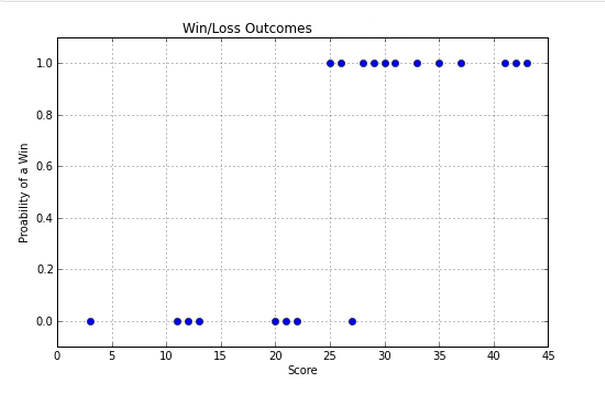
\includegraphics[width=0.6\linewidth]{nfl1}
\end{center}
So, how do we predict whether we have a win or a loss if we are given a score?
\end{frame}



%%%%%%%%%%%%%%%%%%%%%%%%%%%%%%%%%%%%%%%%%%%%%%%%%%%%%%%%%%%%%%%%%%%%%%%%
\begin{frame}[fragile]\frametitle{Game score prediction}
\begin{itemize}
\item Can you fit a line?
\item Sure, you can, but is represent the data?
\item What would be a good representation/model?
\end{itemize}
\end{frame}

%%%%%%%%%%%%%%%%%%%%%%%%%%%%%%%%%%%%%%%%%%%%%%%%%%%%%%%%%%%%%%%%%%%%%%%%
\begin{frame}[fragile]\frametitle{Game score prediction}
Take a look at this plot of a ``best fit'' line over the points.
\begin{center}
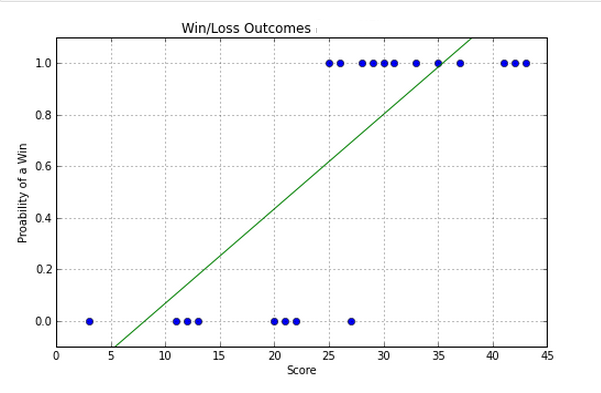
\includegraphics[width=0.6\linewidth]{nfl2}
\end{center}

\end{frame}

%%%%%%%%%%%%%%%%%%%%%%%%%%%%%%%%%%%%%%%%%%%%%%%%%%%%%%%%%%%%%%%%%%%%%%%%
\begin{frame}[fragile]\frametitle{Why not Linear Regression, here?}
\begin{itemize}
\item Probability of winning is bound, from 0 to 1.
\item Scores can range from 0 to 50, say.
\item Now we need a function (or a model) that, given a new score, say, 30. it should compute value between 0 to 1. From the graph, it comes out to be 0.8. Its close to 1, so we can predict that the team will win.
\item Similarly, for score 10, probability is 0.08, very low, so we can predict that the team will lose.
\item But what for scores, 2, or 45. The probabilities are coming out of the range of 0 to 1. Bad!!!
\end{itemize}

\end{frame}

%%%%%%%%%%%%%%%%%%%%%%%%%%%%%%%%%%%%%%%%%%%%%%%%%%%%%%%%%%%%%%%%%%%%%%%%
\begin{frame}[fragile]\frametitle{Why not Linear Regression, here?}
\begin{itemize}
\item Well, we can say, value calculated above 1 is 1, and similarly any value calculated below 0 is considered to be 0. Some sort of Capping.
\item Then the function would look like mirrored ``Z''. It has kinks. Too specific!!, not good.
\item So, clearly linear regression is not a good model.
\item Can we find a better function?
\end{itemize}

\begin{center}
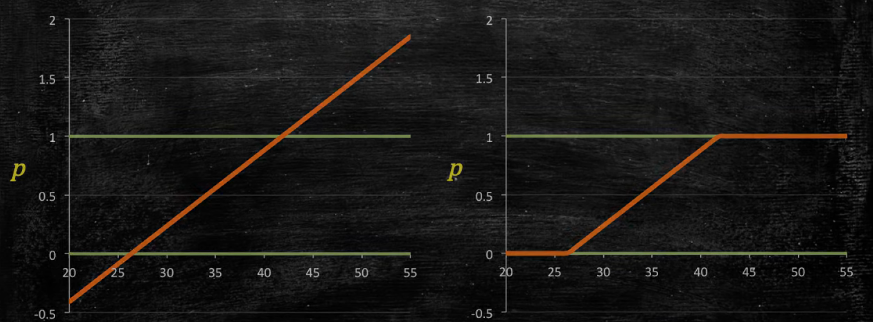
\includegraphics[width=0.6\linewidth]{logreg13}
\end{center}

\end{frame}


%%%%%%%%%%%%%%%%%%%%%%%%%%%%%%%%%%%%%%%%%%%%%%%%%%%%%%%%%%%%%%%%%%%%%%%%
\begin{frame}[fragile]\frametitle{What do we need here?}
\begin{itemize}
\item We need some magic function to represent this requirement. 
\item Input: any number
\item Output: either Boolean or even probabilities between 0 to 1 would do. Using threshold we will convert them to Booleans.
% \item This function will need to have a value of 0 for the loss scores and 1 for the win scores. 
% \item Need a Binary Classifier and not Regression Predictor (score)
% \item Logistic Regression is the solution
\end{itemize}
\end{frame}

%%%%%%%%%%%%%%%%%%%%%%%%%%%%%%%%%%%%%%%%%%%%%%%%%%%%%%%%%%%%%%%%%%%%%%%%
\begin{frame}[fragile]\frametitle{Logistic Regression}
\begin{itemize}
\item For example, consider a logistic regression model for spam detection. 
\item If the model infers a value of 0.932 on a particular email message, it implies a 93.2\% probability that the email message is spam. 
\item More precisely, it means that in the limit of infinite training examples, the set of examples for which the model predicts 0.932 will actually be spam 93.2\% of the time and the remaining 6.8\% will not.
\item Choice of threshold is an important choice, and can be tuned
\end{itemize}

%% (Ref: https://developers.google.com/machine-learning/crash-course/logistic-regression/video-lecture)
\end{frame}


%%%%%%%%%%%%%%%%%%%%%%%%%%%%%%%%%%%%%%%%%%%%%%%%%%%%%%%%%%%%%%%%%%%%%%%%
\begin{frame}[fragile]\frametitle{Logistic Regression}
 \begin{itemize}
\item The name of the Magic function is $logit$.
\item The theory is based on a term called ``Odds''.
\item Lets look at them in details, next.
\end{itemize}

\end{frame}


%%%%%%%%%%%%%%%%%%%%%%%%%%%%%%%%%%%%%%%%%%%%%%%%%%%%%%%%%%%%%%%%%%%%%%%%%%%%%%%%%%
\begin{frame}[fragile]\frametitle{}
\begin{center}
{\Large Background Concepts}
\end{center}
\end{frame}


%%%%%%%%%%%%%%%%%%%%%%%%%%%%%%%%%%%%%%%%%%%%%%%%%%%%%%%%%%%%%%%%%%%%%%%%
\begin{frame}[fragile]\frametitle{Odds vs Probabilities}

\begin{center}
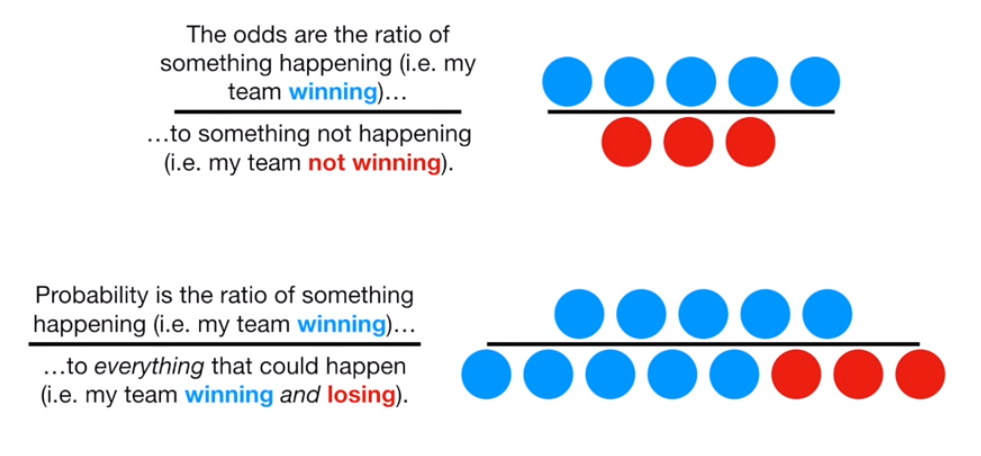
\includegraphics[width=\linewidth,keepaspectratio]{statq51}
\end{center}

\tiny{(Ref: StatQuest: Odds and Log(Odds), Clearly Explained!!! - Josh Starmer )}
\end{frame}


%%%%%%%%%%%%%%%%%%%%%%%%%%%%%%%%%%%%%%%%%%%%%%%%%%%%%%%%%%%%%%%%%%%%%%%%
\begin{frame}[fragile]\frametitle{Odds vs Probabilities}

\begin{center}
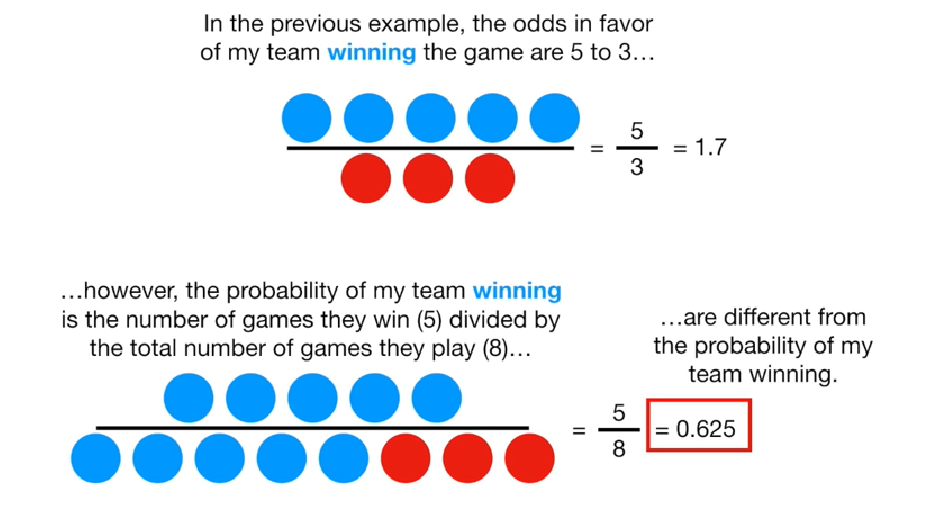
\includegraphics[width=\linewidth,keepaspectratio]{statq52}
\end{center}

\tiny{(Ref: StatQuest: Odds and Log(Odds), Clearly Explained!!! - Josh Starmer )}
\end{frame}



%%%%%%%%%%%%%%%%%%%%%%%%%%%%%%%%%%%%%%%%%%%%%%%%%%%%%%%%%%%%%%%%%%%%%%%%
\begin{frame}[fragile]\frametitle{Probability Basics}

\begin{align}
probability = \frac{one\_outcome}{all\_outcomes} \\
odds = \frac{one\_outcome}{all\_other\_outcomes}
\end{align}
\begin{itemize}
\item Dice roll of 1: probability = 1/6, odds = 1/5
\item Even dice roll: probability = 3/6, odds = 3/3 = 1
\item Dice roll less than 5: probability = 4/6, odds = 4/2 = 2
\end{itemize}
\begin{align}
odds = \frac{probability}{1- probability} \\
probability= \frac{odds }{1+ odds }
\end{align}
\end{frame}

%%%%%%%%%%%%%%%%%%%%%%%%%%%%%%%%%%%%%%%%%%%%%%%%%%%%%%%%%%%%%%%%%%%%%%%%
\begin{frame}[fragile]\frametitle{Odds vs Probabilities}

Lets see how odds can be calculated from Probabilities.

\begin{center}
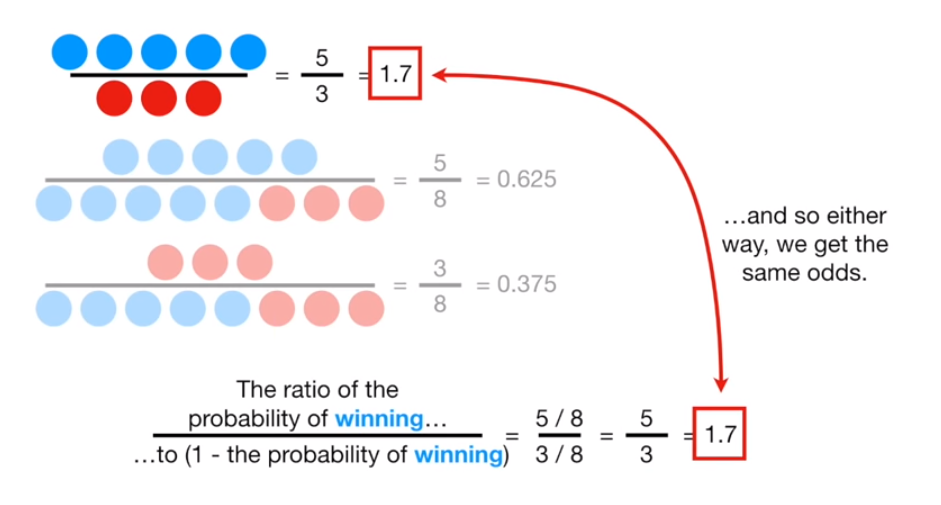
\includegraphics[width=\linewidth,keepaspectratio]{statq53}
\end{center}

So, $odds = \frac{p}{1-p}$
\tiny{(Ref: StatQuest: Odds and Log(Odds), Clearly Explained!!! - Josh Starmer )}
\end{frame}

%%%%%%%%%%%%%%%%%%%%%%%%%%%%%%%%%%%%%%%%%%%%%%%%%%%%%%%%%%%%%%%%%%%%%%%%
\begin{frame}[fragile]\frametitle{Odds vs Probabilities}

Lets take log of odds. But, why?

\begin{itemize}
\item If my team was worse, the odds of winning would be say $\frac{1}{8} = 0.125$
\item If my team was terrible, the odds of winning would be say $\frac{1}{16} = 0.062$
\item If my team was worst, the odds of winning would be say $\frac{1}{32} = 0.031$
\item Worser my team gets the odds get closer to 0. The range is 0 to 1
\item Similarly, for winning, the odds start at 1 and just go up and up, reaching infinity.
\end{itemize}

\begin{center}
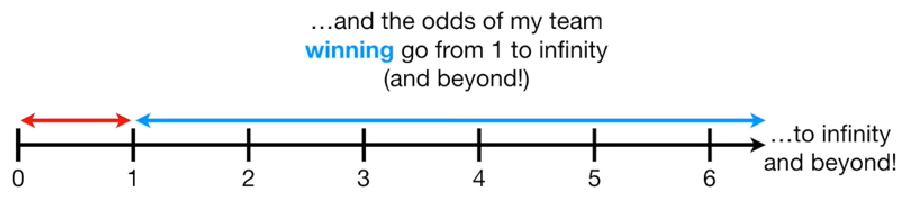
\includegraphics[width=\linewidth,keepaspectratio]{statq54}
\end{center}

This is asymmetrical.

\tiny{(Ref: StatQuest: Odds and Log(Odds), Clearly Explained!!! - Josh Starmer )}
\end{frame}

%%%%%%%%%%%%%%%%%%%%%%%%%%%%%%%%%%%%%%%%%%%%%%%%%%%%%%%%%%%%%%%%%%%%%%%%
\begin{frame}[fragile]\frametitle{Odds vs Probabilities}



\begin{itemize}
\item Asymmetry makes it difficult to compare odds of winning and losing.
\item 1 out of 6, chance on wither side, gives hugely different odds.
\end{itemize}

\begin{center}
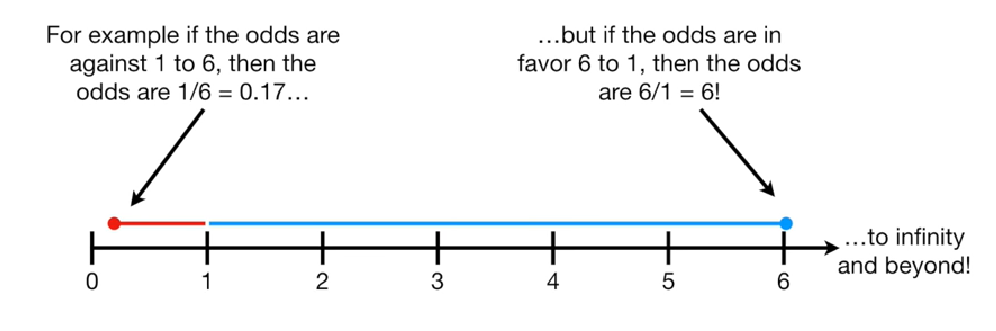
\includegraphics[width=\linewidth,keepaspectratio]{statq55}
\end{center}


\tiny{(Ref: StatQuest: Odds and Log(Odds), Clearly Explained!!! - Josh Starmer )}
\end{frame}


%%%%%%%%%%%%%%%%%%%%%%%%%%%%%%%%%%%%%%%%%%%%%%%%%%%%%%%%%%%%%%%%%%%%%%%%
\begin{frame}[fragile]\frametitle{Odds vs Probabilities}

Taking log of odds, solves this problem by making everything symmetrical.


\begin{center}
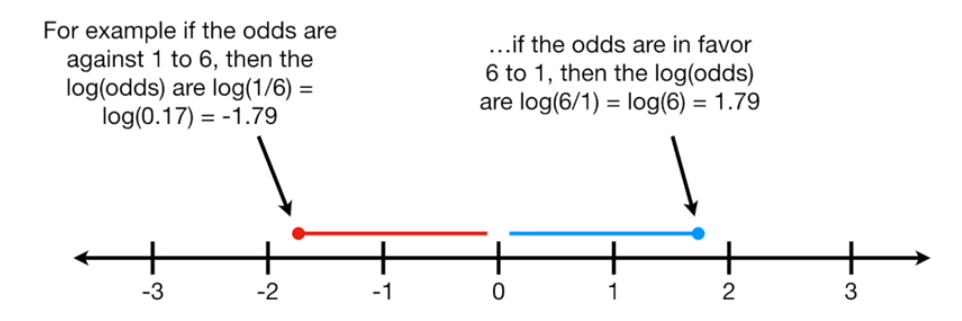
\includegraphics[width=\linewidth,keepaspectratio]{statq56}
\end{center}

Using log, distance from origin  for 6, is same!!
\tiny{(Ref: StatQuest: Odds and Log(Odds), Clearly Explained!!! - Josh Starmer )}
\end{frame}

%%%%%%%%%%%%%%%%%%%%%%%%%%%%%%%%%%%%%%%%%%%%%%%%%%%%%%%%%%%%%%%%%%%%%%%%
\begin{frame}[fragile]\frametitle{Whats the big deal with this log of odds?}

If you pick, random numbers that add up to, say 100 (meaning 20|80, 35|65, this is like winning | losing percentage) and use them to calculate the log(odds) and draw histogram. The histogram is in the shape of normal distribution. The coveted shape of the input data.

\begin{center}
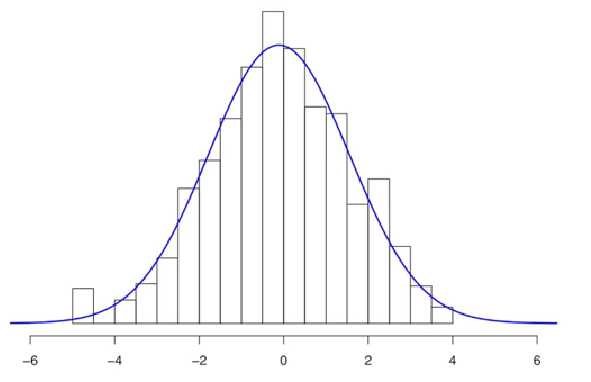
\includegraphics[width=0.6\linewidth,keepaspectratio]{statq57}
\end{center}


\tiny{(Ref: StatQuest: Odds and Log(Odds), Clearly Explained!!! - Josh Starmer )}
\end{frame}

%%%%%%%%%%%%%%%%%%%%%%%%%%%%%%%%%%%%%%%%%%%%%%%%%%%%%%%%%%%%%%%%%%%%%%%%
\begin{frame}[fragile]\frametitle{So, What are Odds? (Summary)}
\begin{center}
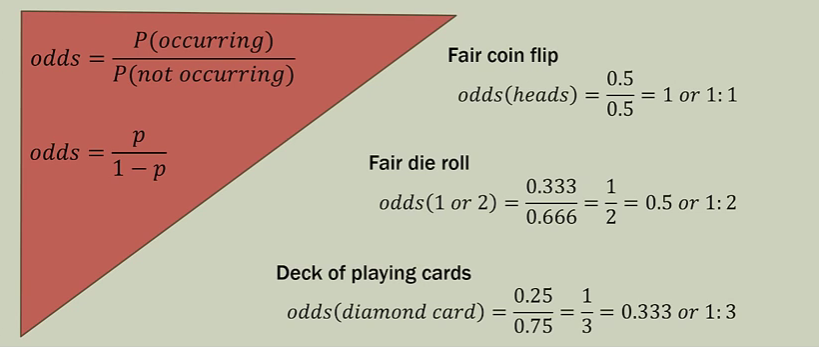
\includegraphics[width=0.9\linewidth]{logregf1}
\end{center}

 \begin{itemize}
\item Odds: Ratio of something happening to that thing not happening.
\item $odds = \frac{p}{(1-p)}$, where, $p$ stands for probability of the positive (the one we want to predict, not necessarily a ``good'' one) event. %Generally for label $y = 1$.
\end{itemize}
\tiny{(Reference: Simple Linear Regression: Step-By-Step - Dan Wellisch)}
\end{frame}


%%%%%%%%%%%%%%%%%%%%%%%%%%%%%%%%%%%%%%%%%%%%%%%%%%%%%%%%%%%%%%%%%%%%%%%%
\begin{frame}[fragile]\frametitle{Logit}
\begin{itemize}
\item $p$ being probability can be only between 0 to 1.% What about range of odds values?
\item Taking log of odds, gives the ``logit'' function $logit(p) = log_e \frac{p}{(1-p)}$
\item Whats the range of logit values?
\end{itemize}
\tiny{(Reference: Simple Linear Regression: Step-By-Step - Dan Wellisch)}
\end{frame}


%%%%%%%%%%%%%%%%%%%%%%%%%%%%%%%%%%%%%%%%%%%%%%%%%%%%%%%%%%%%%%%%%%%%%%%%
\begin{frame}[fragile]\frametitle{Range of Logit}
 \begin{itemize}
\item Put p = 0.5, $logit(0.5) = log \frac{0.5}{(0.5)} = 0$
\item Put p = 0.1, $logit(0.1) = log \frac{0.1}{(0.9)} = -0.95$
\item Put p = 0.01, $logit(0.01) = log \frac{0.01}{(0.99)} = -1.99$
\item Put p = 0.9, $logit(0.9) = log \frac{0.9}{(0.1)} = 0.95$
\item Put p = 0.99, $logit(0.99) = log \frac{0.99}{(0.01)} = 1.99$
\item Put p = 0.999, $logit(0.999) = log \frac{0.999}{(0.001)} = 2.99$
%\item Non linear, dense at ends
\end{itemize}
So, the logit function takes input values in the range 0 to 1 and transforms them to 
values over the entire real number range.
\end{frame}

%%%%%%%%%%%%%%%%%%%%%%%%%%%%%%%%%%%%%%%%%%%%%%%%%%%%%%%%%%%%%%%%%%%%%%%%
\begin{frame}[fragile]\frametitle{Reverse}
We want something inverse \ldots
 \begin{itemize}
\item $logit(p) = log_e \frac{p}{(1-p)}, p = 0 \rightarrow 1$
\item We are interested in reverse
%\item Predicting the probability that a certain 
%sample belongs to a particular class, which is the inverse form of the logit function, which is defined as:

\item $\phi(z) = logit^{-1}(z) = \frac{1}{1+ e^{-z}}, z = -\infty \rightarrow \infty$
\item $z$ is any number. In our case its a linear combination of variables giving any number, and the logit inverse will return the probability
\item $logit^{-1}(z)$ is called as Sigmoid function
\end{itemize}
\end{frame}

%%%%%%%%%%%%%%%%%%%%%%%%%%%%%%%%%%%%%%%%%%%%%%%%%%%%%%%%%%%%%%%%%%%%%%%%
\begin{frame}[fragile]\frametitle{Plotting Sigmoid}
 \begin{lstlisting}
import matplotlib.pyplot as plt
import numpy as np

def sigmoid(z):
	return 1.0 / (1.0 + np.exp(-z))
	
z = np.arange(-7, 7, 0.1)
phi_z = sigmoid(z)
plt.plot(z, phi_z)
plt.axvline(0.0, color='k')
plt.axhspan(0.0, 1.0, facecolor='1.0', alpha=1.0, ls='dotted')
plt.axhline(y=0.5, ls='dotted', color='k')
plt.yticks([0.0, 0.5, 1.0])
plt.ylim(-0.1, 1.1)
plt.xlabel('z')
plt.ylabel('$\phi (z)$')
plt.show() 
\end{lstlisting}
\end{frame}

%%%%%%%%%%%%%%%%%%%%%%%%%%%%%%%%%%%%%%%%%%%%%%%%%%%%%%%%%%%%%%%%%%%%%%%%
\begin{frame}[fragile]\frametitle{Sigmoid}
\begin{center}
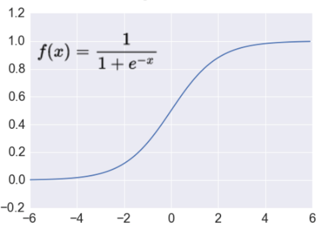
\includegraphics[width=0.6\linewidth]{sigmoid}
\end{center}
\end{frame}

%%%%%%%%%%%%%%%%%%%%%%%%%%%%%%%%%%%%%%%%%%%%%%%%%%%%%%%%%%%%%%%%%%%%%%%%
\begin{frame}[fragile]\frametitle{Sigmoid}
$\phi(z) = logit^{-1}(z) = \frac{1}{1+ e^{-z}}$
 \begin{itemize}
\item If z goes towards infinity then $e^{-z}$ becomes very small , denominator almost 1, thus $\phi(z)$ becomes almost 1. 
\item If z goes towards minus infinity then $e^{-z}$ becomes very large , denominator almost infinity, thus $\phi(z)$ becomes almost 0. 
\item Thus, we conclude that this sigmoid function takes real number values as input and transforms them to values in 
the range [0, 1] with an intercept at  $\phi (z) = 0.5$
\end{itemize}
\end{frame}


%%%%%%%%%%%%%%%%%%%%%%%%%%%%%%%%%%%%%%%%%%%%%%%%%%%%%%%%%%%%%%%%%%%%%%%%%%%%%%%%%%
\begin{frame}[fragile]\frametitle{}
\begin{center}
{\Large Logistic Regression Algorithm}
\end{center}
\end{frame}

%%%%%%%%%%%%%%%%%%%%%%%%%%%%%%%%%%%%%%%%%%%%%%%%%%%%%%%%%%%%%%%%%%%%%%%%
\begin{frame}[fragile]\frametitle{The Magic function}
 \begin{itemize}
\item Example problem, say, that chances of you getting Diabetes is more with age. So, we are finding a function that takes expression $\beta_0 + \beta_1 age$ as input and outputs a probability.
\item For probability, 2 conditions are that the value is always positive and less than 1.
\item Which functions always output positive value given any (positive or negative) value?
\item `Absolute', `Square', etc. One more is exponential.
\item $e^z$ is always positive whatever the $z$ is. But it can be greater than 1.
\item To make it less than 1, lets divide the same term but slightly larger, say, with plus 1. Nice Trick!!
\end{itemize}

\begin{center}
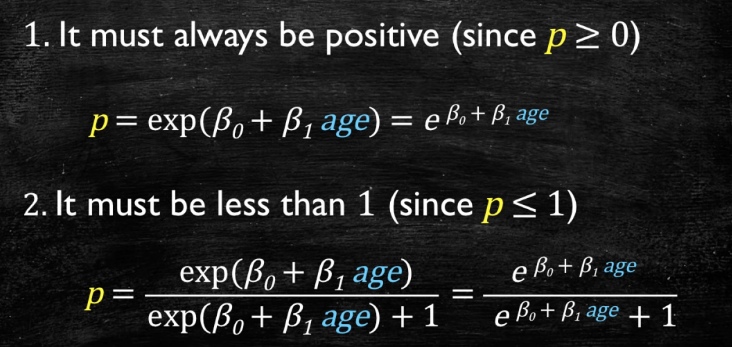
\includegraphics[width=0.6\linewidth]{logreg14}
\end{center}

{\tiny (Ref: Logistic Regression - Interpretation of Coefficients and Forecasting - Data Mining In CAE)}

\end{frame}


%%%%%%%%%%%%%%%%%%%%%%%%%%%%%%%%%%%%%%%%%%%%%%%%%%%%%%%%%%%%%%%%%%%%%%%%
\begin{frame}[fragile]\frametitle{The Magic function}
 \begin{itemize}
\item Rearranging previous equation.
\item Lets say $z = \beta_0 + \beta_1 age$. So we have $p = \frac{e^z}{e^z + 1}$
\item Is it same as $p = \frac{1}{1 + e^{-z}}$? Can not believe? Try.
\item Arranging p terms and taking log on both sides $ln(\frac{p}{1-p}) = z = \beta_0 + \beta_1 age$
\item So even though the probability function is not linear (its exponential), the above arrangement is Linear function of age. Very similar to Linear Regression.
\end{itemize}

\begin{center}
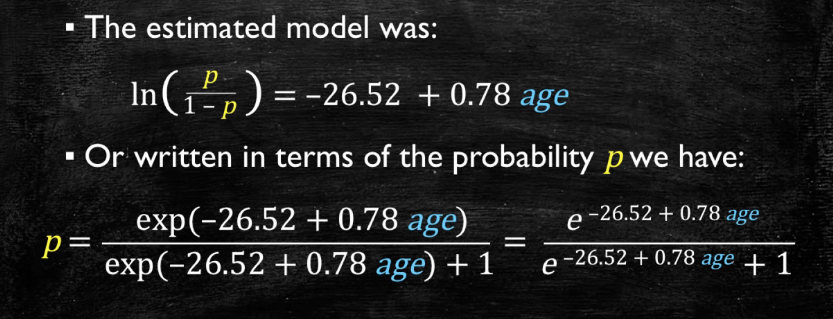
\includegraphics[width=0.6\linewidth]{logreg15}
\end{center}

{\tiny (Ref: Logistic Regression - Interpretation of Coefficients and Forecasting - Data Mining In CAE)}

\end{frame}

%%%%%%%%%%%%%%%%%%%%%%%%%%%%%%%%%%%%%%%%%%%%%%%%%%%%%%%%%%%%%%%%%%%%%%%%
\begin{frame}[fragile]\frametitle{The Magic function}
 \begin{itemize}
\item Plot of Probability vs age looks like a Signmod
\item As the age increases, the chances of getting diabetes are almost equal to 1 (Asymptotic).
\item As the age lowers, the chances of getting diabetes are almost equal to 0 (Asymptotic).
\item $logit(p) = \log(p/(1-p)) = b_0 + b_1 x_1 +  \ldots + b_k x_k$
\item The $ln(\frac{p}{1-p})$ is the logit function and thus the algorithm is called as Logistic.
\item It has Regression expression on the right, so its called Regression.
\item Thus this is Logistic Regression. Used for Classification
\end{itemize}

\begin{center}
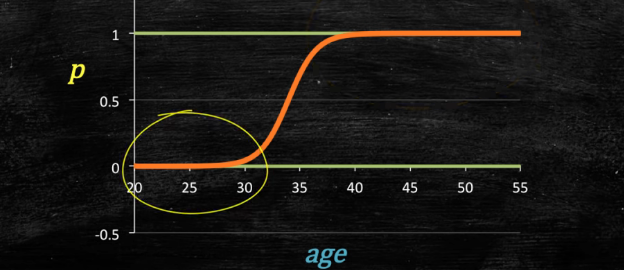
\includegraphics[width=0.6\linewidth]{logreg16}
\end{center}

{\tiny (Ref: Logistic Regression - Interpretation of Coefficients and Forecasting - Data Mining In CAE)}
\end{frame}

%%%%%%%%%%%%%%%%%%%%%%%%%%%%%%%%%%%%%%%%%%%%%%%%%%%%%%%%%%%%%%%%%%%%%%%%
\begin{frame}[fragile]\frametitle{Intuition \ldots}
 \begin{itemize}
\item Whats the meaning of Linear expression's coefficients?
\item In Linear Regression, it meant slope, or proportionality of increase of y wrt x.
\item Here thats not the case.
\item Every unit increase in $age$, $\log(p/(1-p))$ increases $\beta_1$ units.
\item Say, for age as 35, $\beta_0 = -26.52$ and $\beta_1 = 0.78$, the regression comes to be $ = -26,52 + 0.78 \times 35 = 0.813$.
\item Is it Probability of having Diabetes??
\item No. Its logit value.
\item $p = \frac{e^z}{e^z + 1}$ where $z = 0.813$. 
\item Result: Probability $p = 0.693$
\item Approx 70\% chance.
\item Exercise: Calculate for age 36.
\item Confirm: $z = 1.594$ and Probability comes to be 0.831. Just a marginal increase in age, far more chances of getting disease. But after certain age, say 45, the probability settles towards 1.
\end{itemize}
\end{frame}

%%%%%%%%%%%%%%%%%%%%%%%%%%%%%%%%%%%%%%%%%%%%%%%%%%%%%%%%%%%%%%%%%%%%%%%%
\begin{frame}[fragile]\frametitle{Intuition \ldots}
 \begin{itemize}
\item You can add one more variable to the regression part.
\item We add Gender.
\item $z = \beta_0 + \beta_1 age + \beta_1 woman$
\item Assume that betas are calculated and the equation becomes: $z = -26.47 + 0.79 \times age -0.56 \times woman$
\item One year increase in Woman's age increases risk by 14\%, and thats 12\% for male.
\end{itemize}

\begin{center}
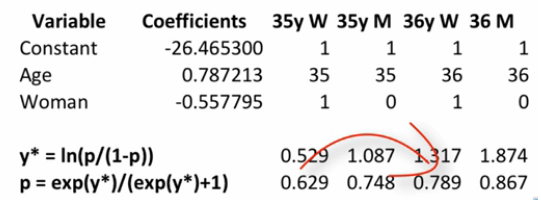
\includegraphics[width=0.6\linewidth]{logreg17}
\end{center}

{\tiny (Ref: Logistic Regression - Interpretation of Coefficients and Forecasting - Data Mining In CAE)}
\end{frame}


%%%%%%%%%%%%%%%%%%%%%%%%%%%%%%%%%%%%%%%%%%%%%%%%%%%%%%%%%%%%%%%%%%%%%%%%
\begin{frame}[fragile]\frametitle{Optimization \ldots}
 \begin{itemize}
\item $logit(p) = \log(p/(1-p)) = b_0 + b_1 x_1 +  \ldots + b_k x_k$

\item Above, p is the probability of presence of the characteristic of interest. 
\item It chooses parameters that maximize  the  likelihood  of  observing  the  sample  values  rather  than  that  minimize  the  sum  of squared errors (like in ordinary regression).
\end{itemize}

\end{frame}

%%%%%%%%%%%%%%%%%%%%%%%%%%%%%%%%%%%%%%%%%%%%%%%%%%%%%%%%%%%%%%%%%%%%%%%%
\begin{frame}[fragile]\frametitle{Conclusion \ldots}
For better understanding \ldots
 \begin{itemize}
 \item So, by now it is clear that the Logistic Regression is somewhat a misnomer!  
\item It  is  a  classification  not  a  regression  algorithm problems.
\item We can imagine that the Logistic Regression is done in two parts.
\item In first, using X features, some intermediate y value is predicted, like Regression.
\item This value is then passed via this Analog to Digital Converter like Sigmoid function, resulting into 0 or 1.
\end{itemize}
\end{frame}



% %%%%%%%%%%%%%%%%%%%%%%%%%%%%%%%%%%%%%%%%%%%%%%%%%%%%%%%%%%%%%%%%%%%%%%%%
% \begin{frame}[fragile]\frametitle{Logistic Regression}
% \begin{itemize}
% \item The linear regression model with one variable: $y = mx + c$
% \item The logistic regression model with one variable: $logit(p) = mx + c$, where $logit(p) = ln(\frac{p}{1-p})$
% \item So, logistic regression: Given value of the independent variables, the regression equation predicts Log Odds Ratio
% \end{itemize}
% \end{frame}

% %%%%%%%%%%%%%%%%%%%%%%%%%%%%%%%%%%%%%%%%%%%%%%%%%%%%%%%%%%%%%%%%%%%%%%%%
% \begin{frame}[fragile]\frametitle{Logistic Regression}
% \begin{itemize}
% \item So, Logistic regression can be viewed as an extension of linear regression to classification problems. 
% \item One of the limitations of linear regression is that it cannot provide class probability estimates. 
% \item This is often useful, for example, when we want to inspect manually the most fraudulent cases. 
% \end{itemize}
% \end{frame}

% %%%%%%%%%%%%%%%%%%%%%%%%%%%%%%%%%%%%%%%%%%%%%%%%%%%%%%%%%%%%%%%%%%%%%%%%
% \begin{frame}[fragile]\frametitle{Logistic Regression}
% \begin{itemize}
% \item Basically, we would like to constrain the predictions of the model to the range $[0,1]$ so that we can interpret them as probability estimates. 
% \item In Logistic Regression, we use the logit function to clamp predictions from the range $[-infty,infty]$ to $[0,1]$. 
% \end{itemize}
% \end{frame}



% %%%%%%%%%%%%%%%%%%%%%%%%%%%%%%%%%%%%%%%%%%%%%%%%%%%%%%%%%%%%%%%%%%%%%%%%
% \begin{frame}[fragile]\frametitle{Logistic Regression -- Predictions}
% \begin{center}
% 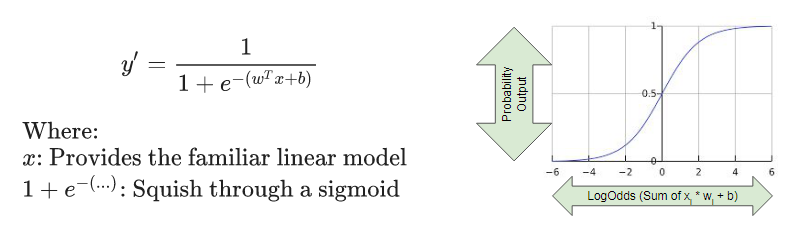
\includegraphics[width=\linewidth]{logistic1}
% \end{center}
% Logistic Function: outputs between 0 and 1 for all values of X


% $y' = \frac{e^t}{e^t + 1} = \frac{1}{1 + e^{-t}}$

% % % (Ref: https://developers.google.com/machine-learning/crash-course/logistic-regression/video-lecture)
% \end{frame}

%%%%%%%%%%%%%%%%%%%%%%%%%%%%%%%%%%%%%%%%%%%%%%%%%%%%%%%%%%%%%%%%%%%%%%%%%
%\begin{frame}[fragile]\frametitle{Logistic Transformation}
%\begin{center}
%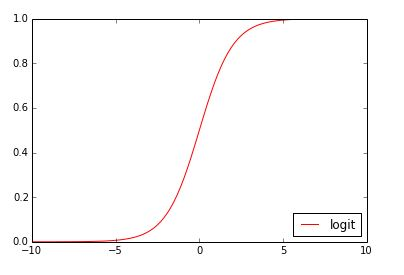
\includegraphics[width=\linewidth]{sklclass13}
%\end{center}
%\end{frame}


% %%%%%%%%%%%%%%%%%%%%%%%%%%%%%%%%%%%%%%%%%%%%%%%%%%%%%%%%%%%%%%%%%%%%%%%%
% \begin{frame}[fragile]\frametitle{Logit Function}
% \begin{itemize}
% \item Values of the odds close to 0 indicate very low probabilities
% \item High odds indicate very high probabilities.
% \end{itemize}
% \begin{center}
% 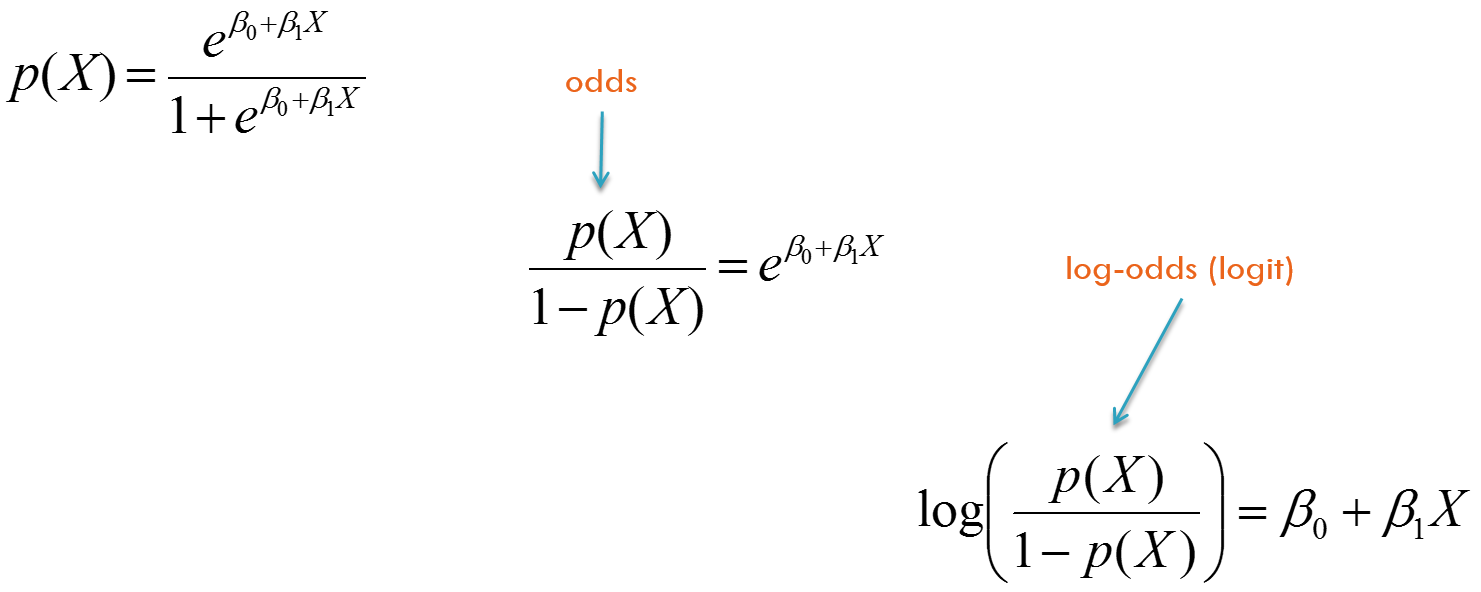
\includegraphics[width=\linewidth]{logit}
% \end{center}
% Logit is linear in X

% \end{frame}

%
%%%%%%%%%%%%%%%%%%%%%%%%%%%%%%%%%%%%%%%%%%%%%%%%%%%%%%%%%%%%%%%%%%%%%%%%%
%\begin{frame}[fragile]\frametitle{Interpretation}
%\begin{center}
%
\includegraphics[width=0.7\linewidth]{loglineq}
%\end{center}
%\begin{itemize}
%\item Linear
%	\begin{itemize}
%	\item $\beta_1$ gives the average change in Y with a one-unit increase in X'
%	\item Relationship is constant (straight line)
%	\end{itemize}
%\item Logistic
%	\begin{itemize}
%	\item Increasing X by one unit changes the log odds by $\beta_1$, (multiplies the odds by $e^{\beta_1}$)
%	\item Relationship is not a straight line. The amount that Y changes depends on the current value of X
%	\end{itemize}
%\item Maximum likelihood is used (instead of least squares)
%\item scikit calculates ``best'' coefficients automatically for us
%\end{itemize}
%
%\end{frame}


%%%%%%%%%%%%%%%%%%%%%%%%%%%%%%%%%%%%%%%%%%%%%%%%%%%%%%%%%%%%%%%%%%%%%%%%%%%%%%%%%%
\begin{frame}[fragile]\frametitle{}
\begin{center}
{\Large Hyperplane Approach (Advance)}
\end{center}

{\tiny (Ref: Logistic Regression (for dummies) - Sachin Joglekar)}
\end{frame}

%%%%%%%%%%%%%%%%%%%%%%%%%%%%%%%%%%%%%%%%%%%%%%%%%%%%%%%%%%%%%%%%%%%%%%%%
\begin{frame}[fragile]\frametitle{Logistic Regression}
\begin{itemize}
\item Unlike actual regression, logistic regression does not try to predict the value of a numeric variable given a set of inputs. Instead, the output is a probability that the given input point belongs to a certain class.
\item  Your input space can be separated into two nice regions, one for each class, by a linear(read: straight) boundary.

\item Equation of the separating Hyperplane is given by $W^Tx = 0$ 

\item Whereas $W^Tx$ gives a distance of a $x$ point from $W^Tx = 0$ Hyperplane.
\end{itemize}

\end{frame}

%%%%%%%%%%%%%%%%%%%%%%%%%%%%%%%%%%%%%%%%%%%%%%%%%%%%%%%%%%%%%%%%%%%%%%%%
\begin{frame}[fragile]\frametitle{Logistic Regression Visualization}
\begin{center}
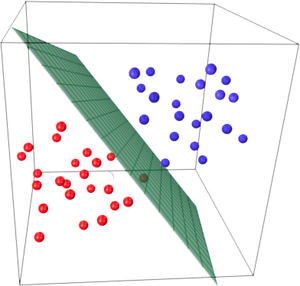
\includegraphics[width=0.5\linewidth]{logreg1}
\end{center}

$W^Tx = 0$ is a generalization for $n$ dimensions with both $w$ and $x$ as n dimensional vectors and the Hyperplane is the dot product.

{\tiny (Ref: http://blog.sairahul.com/2014/01/linear-separability.html)}
\end{frame}


%%%%%%%%%%%%%%%%%%%%%%%%%%%%%%%%%%%%%%%%%%%%%%%%%%%%%%%%%%%%%%%%%%%%%%%%
\begin{frame}[fragile]\frametitle{Logistic Regression}
Lets look at 2D example, as a special, simpler case:
\begin{itemize}
\item Let there be 1 input variable $x_1$ and output variable $y$, is now called as $x_2$ (just renaming, for convenience, to be appreciated later !!)

\item So equation of line becomes $x_2 = kx_1 + B$ thus $kx_1 -x_2 + B =0$
\end{itemize}

\begin{center}
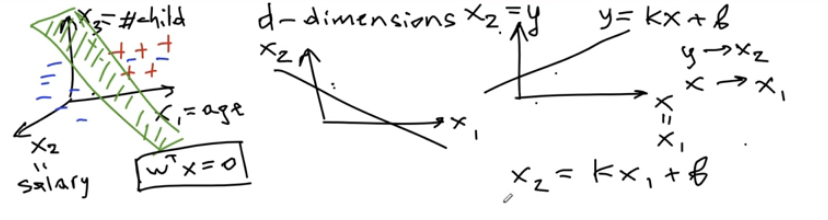
\includegraphics[width=0.9\linewidth]{logreg2}
\end{center}

{\tiny (Ref: mlcourse.ai. Lecture 4. Logistic regression. Theory)}

\end{frame}


%%%%%%%%%%%%%%%%%%%%%%%%%%%%%%%%%%%%%%%%%%%%%%%%%%%%%%%%%%%%%%%%%%%%%%%%
\begin{frame}[fragile]\frametitle{Logistic Regression}
\begin{itemize}
\item $kx_1 -x_2 + B =0$ can be represented as $W^Tx = 0$ where $W = [B, k, -1]$ as column vector and $x =  [1 x_1 x_2]$ also as column vector.
\item The dot product $(3 \times 1)^T \times (3 \times 1) = 1 \times 1$ gives the expression $kx_1 -x_2 + B =0$

\item $x$ can be extended to $n$ dimensions. Then $W^Tx = 0$ becomes equation of Hyperplane.
\end{itemize}

\begin{center}
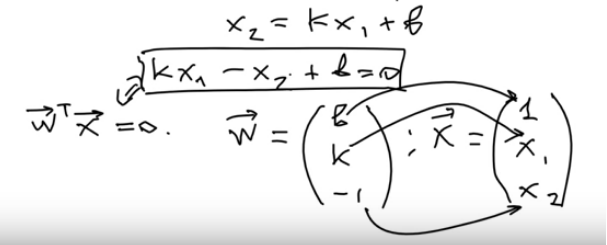
\includegraphics[width=0.7\linewidth]{logreg3}
\end{center}

{\tiny (Ref: mlcourse.ai. Lecture 4. Logistic regression. Theory)}

\end{frame}

%%%%%%%%%%%%%%%%%%%%%%%%%%%%%%%%%%%%%%%%%%%%%%%%%%%%%%%%%%%%%%%%%%%%%%%%
\begin{frame}[fragile]\frametitle{Logistic Regression}
\begin{itemize}
\item Hyperplane $W^Tx = 0$ separates + and - data points, meaning space into 2 regions.
\item In one region, for those data points (meaning, x values) $W^Tx > 0$ and in the other the data points' x values will evaluate $W^Tx < 0$
\item Once training is done, $W$ is ready, for a new point, we will evaluate $W^Tx$ and see if its less or more or equal to 0 and classify accordingly as = or -.
\end{itemize}

\begin{center}
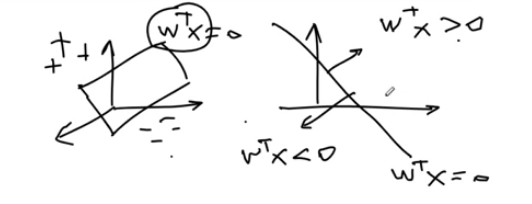
\includegraphics[width=0.5\linewidth]{logreg4}
\end{center}

(Note: In some cases data points may be such that, the hyperplane may not be able to separate + and - points perfectly. There will be some mis-classifications. Thats OK.)

{\tiny (Ref: mlcourse.ai. Lecture 4. Logistic regression. Theory)}

\end{frame}

%%%%%%%%%%%%%%%%%%%%%%%%%%%%%%%%%%%%%%%%%%%%%%%%%%%%%%%%%%%%%%%%%%%%%%%%
\begin{frame}[fragile]\frametitle{Logistic Regression}
\begin{itemize}

\item $W^Tx$ is actually a distance of point A ie $x_A$ from the hyperplane. Just need to divide by norm, so the distance $\rho = \frac{W^Tx_A}{||W||}$, where $||W||$ is $L_2$ norm given by $\sqrt{W_0^2 + W_1^2 + \ldots}$
\item $\rho$ can be positive and negative, different for different point. Thus classification.
\end{itemize}

\begin{center}
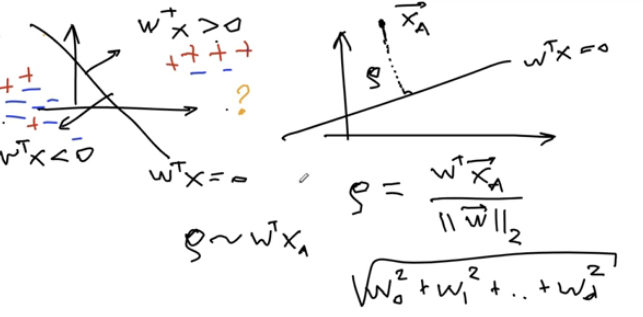
\includegraphics[width=0.7\linewidth]{logreg5}
\end{center}

{\tiny (Ref: mlcourse.ai. Lecture 4. Logistic regression. Theory)}

\end{frame}


%%%%%%%%%%%%%%%%%%%%%%%%%%%%%%%%%%%%%%%%%%%%%%%%%%%%%%%%%%%%%%%%%%%%%%%%
\begin{frame}[fragile]\frametitle{Logistic Regression - Geometrical Background}

\begin{itemize}
\item But we don't want to just predict sign (+ or -) but how much + or how much -, ie we want probabilities of the sign.
\item Very useful in cases such as Loan customer is good or bad and also how much. We can sort by probabilities and then disburse loan. Probabilities give ratings.
\end{itemize}

\end{frame}



%%%%%%%%%%%%%%%%%%%%%%%%%%%%%%%%%%%%%%%%%%%%%%%%%%%%%%%%%%%%%%%%%%%%%%%%
\begin{frame}[fragile]\frametitle{Logistic Regression}

So the classifier is $a(\textbf{x}) = \text{sign}(\textbf{w}^\text{T}\textbf x),$ where
 \begin{itemize}
 \item $x$ – is a feature vector (along with identity);
\item $w$ – is a vector of weights in the linear model (with bias w0);
\item $\text{sign}(\bullet)$ – is the signum function that returns the sign of its argument;
\item $a(x)$ – is a classifier response for $x$.
  \end{itemize}
\end{frame}


%%%%%%%%%%%%%%%%%%%%%%%%%%%%%%%%%%%%%%%%%%%%%%%%%%%%%%%%%%%%%%%%%%%%%%%%
\begin{frame}[fragile]\frametitle{Logistic Regression}
 \begin{itemize}
 \item So, Logistic regression is a special case of the linear classifier, but it has an added benefit of predicting a probability $p_+$ of referring example $x_i$ to the class ``+'': $\Large p_+ = P\left(y_i = 1 \mid \textbf{x}_\text{i}, \textbf{w}\right)$
 \item Being able to predict not just a response ( "+1" or "-1") but the probability of assignment to class "+1" is a very important requirement in many business problems 
 \item E.g. credit scoring where logistic regression is traditionally used. 
 \item Customers who have applied for a loan are ranked based on this predicted probability (in descending order) to obtain a scoreboard that rates customers from bad to good.
\end{itemize}

\end{frame}


%%%%%%%%%%%%%%%%%%%%%%%%%%%%%%%%%%%%%%%%%%%%%%%%%%%%%%%%%%%%%%%%%%%%%%%%
\begin{frame}[fragile]\frametitle{Logistic Regression}
Below is an example of such a toy scoreboard.
\begin{center}
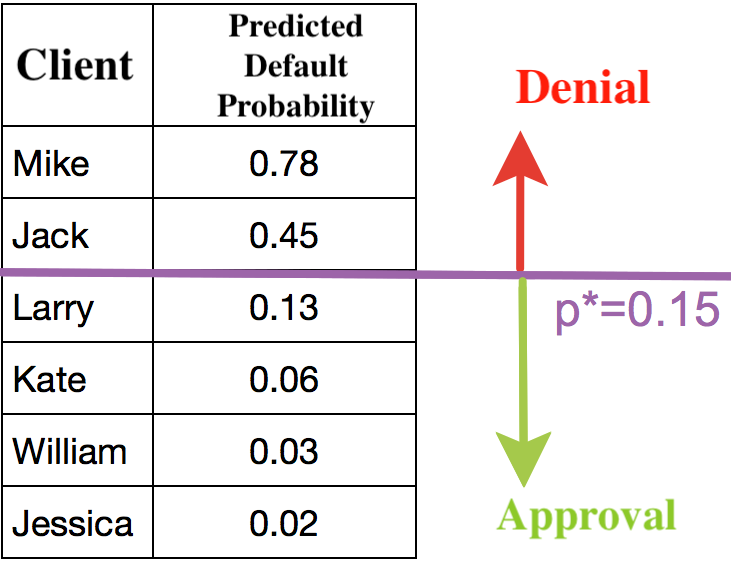
\includegraphics[width=0.35\linewidth]{mlcourse20}
\end{center}
 \begin{itemize}
 \item The bank chooses a threshold $p_*$ to predict the probability of loan default (in the picture it's 0.15) and stops approving loans starting from that value. 
 \item Moreover, it is possible to multiply this predicted probability by the loan amount to get the expectation of losses from the client, which can also constitute good business metrics.
 \end{itemize}

\end{frame}

%%%%%%%%%%%%%%%%%%%%%%%%%%%%%%%%%%%%%%%%%%%%%%%%%%%%%%%%%%%%%%%%%%%%%%%%
\begin{frame}[fragile]\frametitle{Logistic Regression - Probability calculation}
\begin{itemize}
\item To predict the probability $p_+ \in [0,1]$, we can start by constructing a linear prediction using OLS: $b(\textbf{x}) = \textbf{w}^\text{T} \textbf{x} \in \mathbb{R}$. But converting the resulting value to the probability within in the [0, 1] range requires some function $f: \mathbb{R} \rightarrow [0,1]$. Logistic regression uses a specific function for this: $\sigma(z) = \frac{1}{1 + \exp^{-z}}$. 
\end{itemize}

\begin{center}
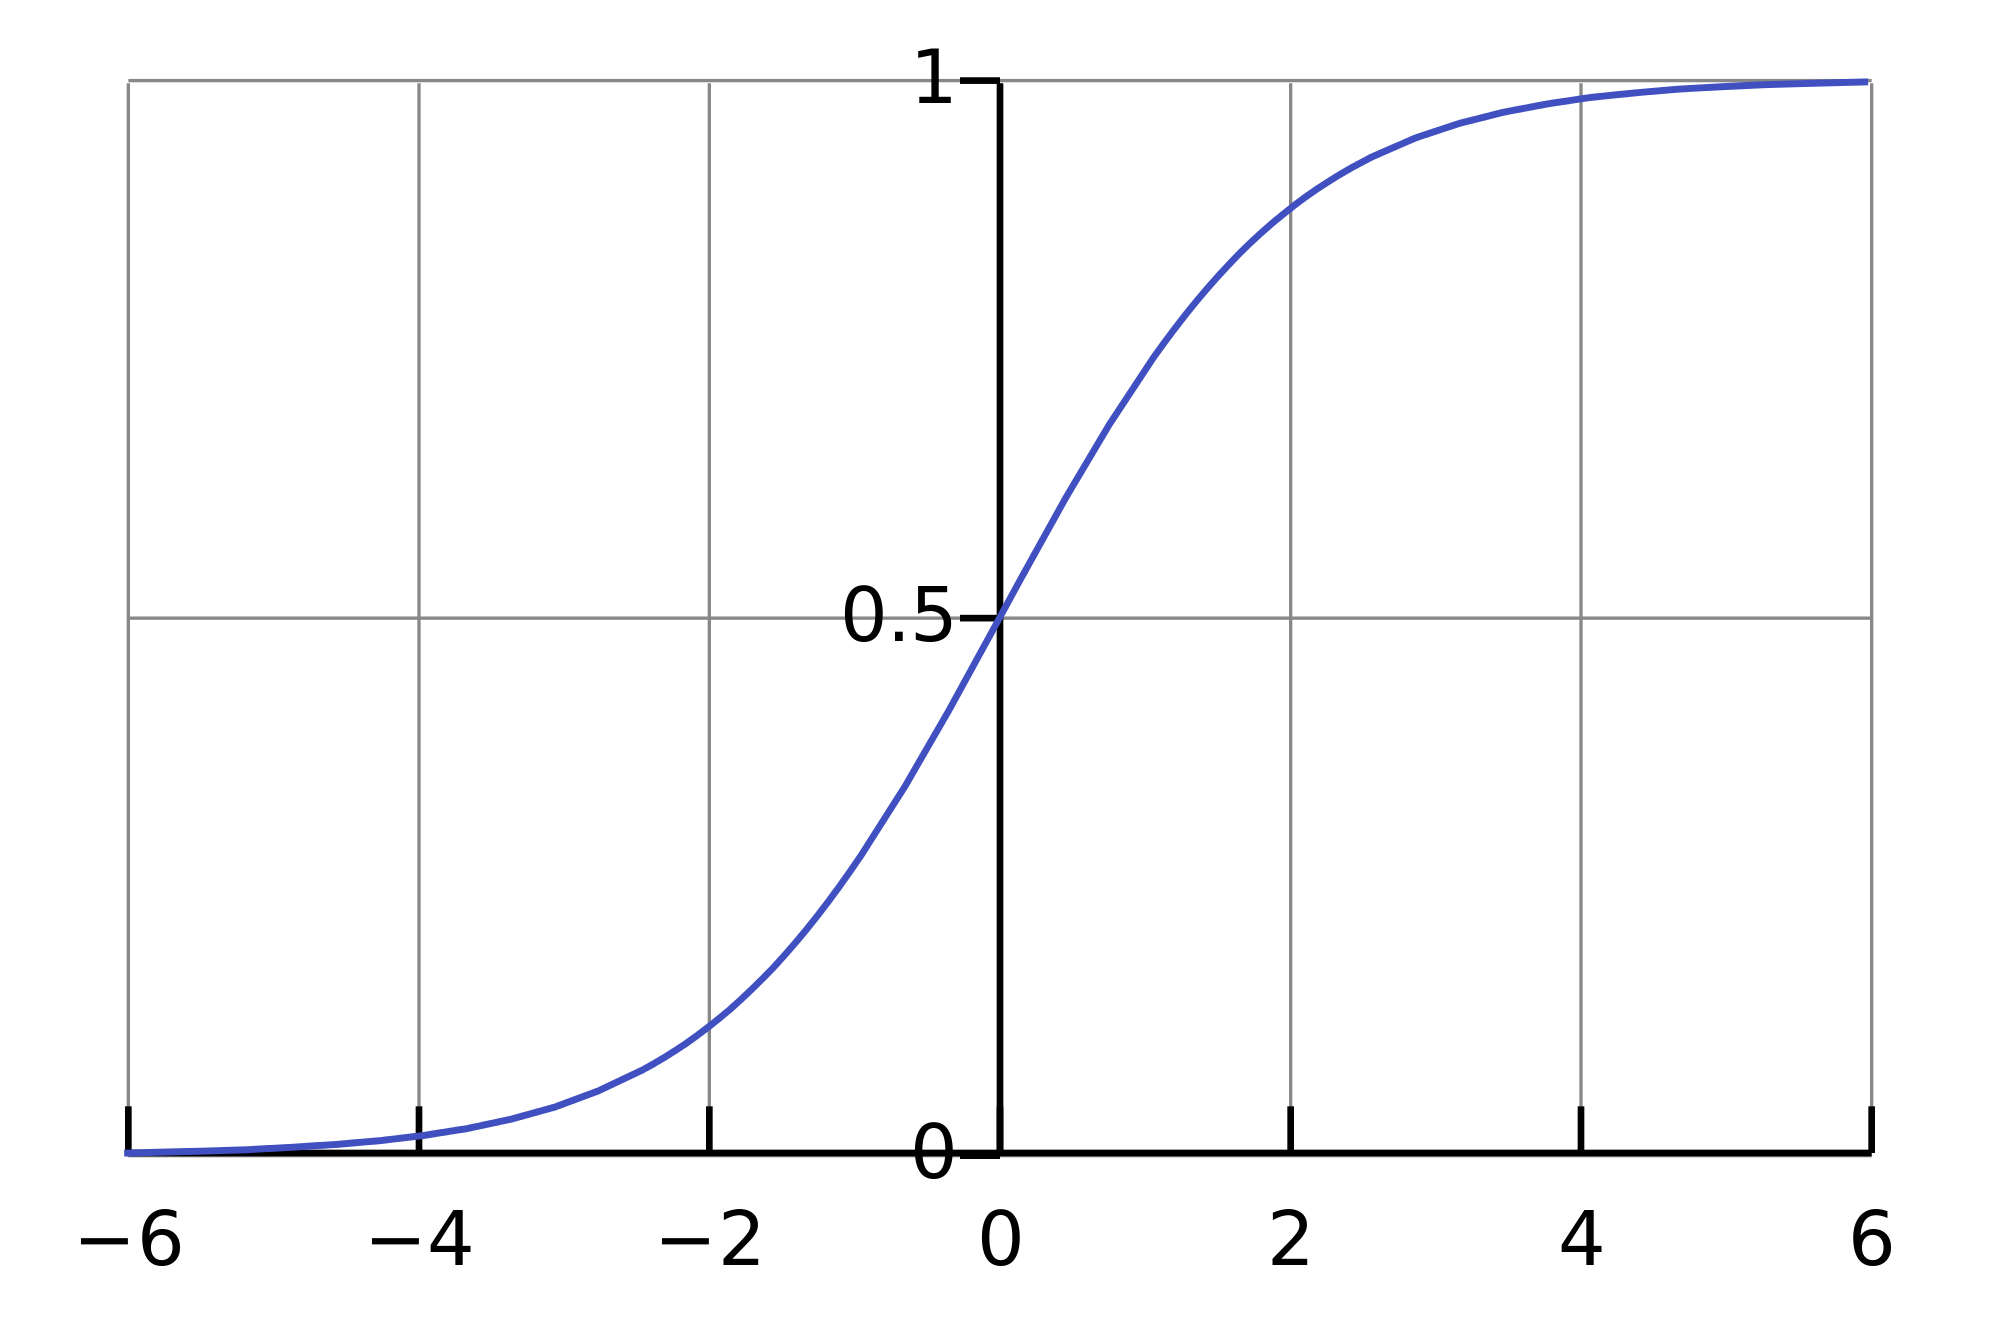
\includegraphics[width=0.35\linewidth]{mlcourse24}
\end{center}

\end{frame}


%%%%%%%%%%%%%%%%%%%%%%%%%%%%%%%%%%%%%%%%%%%%%%%%%%%%%%%%%%%%%%%%%%%%%%%%
\begin{frame}[fragile]\frametitle{Logistic Regression - Probability calculation}
Lets take an example:
\begin{itemize}
\item Assuming two input variables for simplicity(unlike the 3-dimensional figure shown before)- $x_1$ and $x_2$, the function corresponding to the boundary will be something like $\beta_0 + \beta_1 x_1 + \beta_2 x_2$.

\item It is crucial to note that $x_1$ and $x_2$ are BOTH input variables, and the output variable isn't a part of the conceptual space- unlike a technique like linear regression.
\end{itemize}

\end{frame}


%%%%%%%%%%%%%%%%%%%%%%%%%%%%%%%%%%%%%%%%%%%%%%%%%%%%%%%%%%%%%%%%%%%%%%%%
\begin{frame}[fragile]\frametitle{Logistic Regression - Geometrical Background}
\begin{itemize}
\item Consider a point $(a, b)$. Plugging the values of  $x_1$ and $x_2$ into the boundary function, we will get its output $\beta_0 + \beta_1 a + \beta_2 b$.

\item Now depending on the location of $(a, b)$, there are three possibilities to consider: \ldots

\end{itemize}

\end{frame}

%%%%%%%%%%%%%%%%%%%%%%%%%%%%%%%%%%%%%%%%%%%%%%%%%%%%%%%%%%%%%%%%%%%%%%%%
\begin{frame}[fragile]\frametitle{Logistic Regression - Geometrical Background}
I:
\begin{itemize}
\item $(a, b)$ lies in the region defined by points of the + class. 
\item As a result, $\beta_0 + \beta_1 a + \beta_2 b$ will be positive, lying somewhere in $(0, \infty)$. 
\item Mathematically, the higher the magnitude of this value, the greater is the distance between the point and the boundary. 
\item Intuitively speaking, the greater is the probability that $(a, b)$ belongs to the + class. Therefore, $P_+$ will lie in $(0.5, 1]$.

\end{itemize}

\end{frame}

%%%%%%%%%%%%%%%%%%%%%%%%%%%%%%%%%%%%%%%%%%%%%%%%%%%%%%%%%%%%%%%%%%%%%%%%
\begin{frame}[fragile]\frametitle{Logistic Regression - Geometrical Background}
II:
\begin{itemize}
\item $(a, b)$ lies in the region defined by points of the - class. 
\item Now, $\beta_0 + \beta_1 a + \beta_2 b$ will be negative, lying in $(-\infty, 0)$. 
\item But like in the positive case, higher the absolute value of the function output, greater the probability that $(a, b)$ belongs to the - class. $P_+$ will now lie in [0, 0.5).

\end{itemize}

\end{frame}

%%%%%%%%%%%%%%%%%%%%%%%%%%%%%%%%%%%%%%%%%%%%%%%%%%%%%%%%%%%%%%%%%%%%%%%%
\begin{frame}[fragile]\frametitle{Logistic Regression - Geometrical Background}
III:
\begin{itemize}
\item $(a, b)$ lies ON the linear boundary. 
\item In this case, $\beta_0 + \beta_1 a + \beta_2 b = 0$. 
\item This means that the model cannot really say whether $(a, b)$ belongs to the + or - class. 
\item As a result, $P_+$ will be exactly 0.5.

\end{itemize}

\end{frame}

%%%%%%%%%%%%%%%%%%%%%%%%%%%%%%%%%%%%%%%%%%%%%%%%%%%%%%%%%%%%%%%%%%%%%%%%
\begin{frame}[fragile]\frametitle{Logistic Regression - Geometrical Background}

\begin{itemize}
\item  In $a(\textbf{x}) = \text{sign}(\textbf{w}^\text{T}\textbf x)$, $x$ is a vector like $x = (1, x_1,x_2,\ldots)$, where $x_0$ is typically taken as a constant, a bias, say, 1. These $x$ features can be, say, Salary, Age, etc.
\item $W$ is also set of values like $W = (w_0, w_a,w_2,\ldots)$ these are like coefficients in standard linear equation.
\item Resultant is a real number between $-\infty$ to $\infty$.
\item So now we have a function that outputs a value in $(-\infty, \infty)$ given an input data point. \item But how do we map this to the probability  $P_+$, that goes from [0, 1]? 
\item The answer, is in the odds function (seen before).
\end{itemize}

\end{frame}

%%%%%%%%%%%%%%%%%%%%%%%%%%%%%%%%%%%%%%%%%%%%%%%%%%%%%%%%%%%%%%%%%%%%%%%%
\begin{frame}[fragile]\frametitle{Logistic Regression - Geometrical Background}
The Trick:
\begin{itemize}
\item 
Let $P(X)$ denote the probability of an event $X$ occurring. 
\item In that case, the odds ratio $(OR(X))$ is defined by  $\frac{P(X)}{1-P(X)}$, which is essentially the ratio of the probability of the event happening, vs. it not happening. 
\item It is clear that probability and odds convey the exact same information. But as $P(X)$ goes from 0 to 1, $OR(X)$ goes from 0 to $\infty$.
\item 
However, we are still not quite there yet, since our boundary function gives a value from $–\infty to \infty$. So what we do, is take the logarithm of $OR(X)$, called the log-odds function. 
\item Mathematically, as $OR(X)$ goes from 0 to $\infty$, $log(OR(X))$ goes from $–\infty to \infty$!

\end{itemize}

\end{frame}

%%%%%%%%%%%%%%%%%%%%%%%%%%%%%%%%%%%%%%%%%%%%%%%%%%%%%%%%%%%%%%%%%%%%%%%%
\begin{frame}[fragile]\frametitle{Logistic Regression - Geometrical Background}
The Trick:
\begin{itemize}
\item Main idea of the Logistic Regression is to be able to predict $OR(X)$ with just $\textbf{w}^\text{T}\textbf x$
\item Now we can say $log(OR_+) = \textbf{w}^\text{T}\textbf x$ as both are from $–\infty to \infty$ and once we equate, we are essentially putting $y = f(x)$, thus, then, the weights could be found out during Training.
\item Expanding $OR_+$ we get $log (\frac{P_+}{1-P_+}) = \textbf{w}^\text{T}\textbf x$
\item Taking 'log' to other side as $e$, the equation becomes $P_+ = \frac{e^{\textbf{w}^\text{T}\textbf x}}{1+ e^{\textbf{w}^\text{T}\textbf x}} = \frac{1}{1 + e^{-\textbf{w}^\text{T}\textbf x}}$
\item This is Sigmoid function $\sigma(z) = \frac{1}{1+e^{-z}}$
\end{itemize}

\end{frame}


%%%%%%%%%%%%%%%%%%%%%%%%%%%%%%%%%%%%%%%%%%%%%%%%%%%%%%%%%%%%%%%%%%%%%%%%
\begin{frame}[fragile]\frametitle{Logistic Regression - Geometrical Background}
Finally:
\begin{itemize}
\item 
We have a way to interpret the result of plugging in the attributes of an input into the boundary function. 
\item The boundary function actually defines the log-odds of the + class, in our model. 
\item So essentially, in our two-dimensional example, given a point $(a, b)$, this is what Logistic regression would do.

\end{itemize}

\end{frame}

%%%%%%%%%%%%%%%%%%%%%%%%%%%%%%%%%%%%%%%%%%%%%%%%%%%%%%%%%%%%%%%%%%%%%%%%
\begin{frame}[fragile]\frametitle{Logistic Regression Steps}
Let's see how logistic regression will make a prediction $p_+ = P\left(y_i = 1 \mid \textbf{x}_\text{i}, \textbf{w}\right)$. (For now, let's assume that we have somehow obtained weights w i.e. trained the model)
 \begin{itemize}
 
\item Step 1. Calculate $w_{0}+w_{1}x_1 + w_{2}x_2 + ... = \textbf{w}^\text{T}\textbf{x}$. (Equation $\textbf{w}^\text{T}\textbf{x} = 0$ defines a hyperplane separating the examples into two classes);

\item Step 2. Compute the log odds ratio: $\log(OR_{+}) = \textbf{w}^\text{T}\textbf{x}$
\end{itemize}

\end{frame}

%%%%%%%%%%%%%%%%%%%%%%%%%%%%%%%%%%%%%%%%%%%%%%%%%%%%%%%%%%%%%%%%%%%%%%%%
\begin{frame}[fragile]\frametitle{Logistic Regression Steps}
 \begin{itemize}

\item Step 3. Now that we have the chance of assigning an example to the class of "+" - $OR_{+}$, calculate $p_{+}$ using the simple relationship:
$ p_{+} = \frac{OR_{+}}{1 + OR_{+}} = \frac{\exp^{\textbf{w}^\text{T}\textbf{x}}}{1 + \exp^{\textbf{w}^\text{T}\textbf{x}}} = \frac{1}{1 + \exp^{-\textbf{w}^\text{T}\textbf{x}}} = \sigma(\textbf{w}^\text{T}\textbf{x})$
\item On the right side, you can see that we have the sigmoid function.
\end{itemize}

\end{frame}



%%%%%%%%%%%%%%%%%%%%%%%%%%%%%%%%%%%%%%%%%%%%%%%%%%%%%%%%%%%%%%%%%%%%%%%%
\begin{frame}[fragile]\frametitle{Logistic Regression Steps}
 \begin{itemize}

\item So, logistic regression predicts the probability of assigning an example to the "+" class (assuming that we know the features and weights of the model) as a sigmoid transformation of a linear combination of the weight vector and the feature vector:
$ p_+(\textbf{x}_\text{i}) = P\left(y_i = 1 \mid \textbf{x}_\text{i}, \textbf{w}\right) = \sigma(\textbf{w}^\text{T}\textbf{x}_\text{i}).$
\item Next, we will see how the model is trained. We will again rely on maximum likelihood estimation.
\end{itemize}

\end{frame}

%%%%%%%%%%%%%%%%%%%%%%%%%%%%%%%%%%%%%%%%%%%%%%%%%%%%%%%%%%%%%%%%%%%%%%%%%%%%%%%%%%
\begin{frame}[fragile]\frametitle{}
\begin{center}
{\Large Maximum Likelihood Estimation (Advance)}
\end{center}
\end{frame}


%%%%%%%%%%%%%%%%%%%%%%%%%%%%%%%%%%%%%%%%%%%%%%%%%%%%%%%%%%%%%%%%%%%%%%%%
\begin{frame}[fragile]\frametitle{Maximum Likelihood Estimation (MLE) Intuition}
Example
 \begin{itemize}
\item If you are passing by a Shop everyday at around 2 pm, and you see that the shop is closed (you are in Pune!!!), 
\item Then maximum likelihood estimate would be that the shop will be closed when you pass by tomorrow 1 pm.
\item This MLE approach is often used to fit distributions in observed data.
\item Distribution is what you see when you plot Histogram of observed data, ie data values on x axis and frequencies of occurrences of each data values on y axis.
\item Once you fit the distribution, say Normal Distribution, you get parameters $\mu$ and $\sigma$
\end{itemize}

\end{frame}

%%%%%%%%%%%%%%%%%%%%%%%%%%%%%%%%%%%%%%%%%%%%%%%%%%%%%%%%%%%%%%%%%%%%%%%%
\begin{frame}[fragile]\frametitle{Maximum Likelihood Estimation (MLE) Intuition}
In logistic regression, we will estimate W's with MLE. How?
\begin{itemize}
\item $P = \{y=y_i | x_i;W\} = Sigmoid(y_i W^Tx_i)$ is a cleaver combination for $y = \pm 1$

\item MLE is for maximizing probability of observing vector $y$ given that we observer matrix $X$ and parameters matrix $W$.
\end{itemize}


\begin{center}
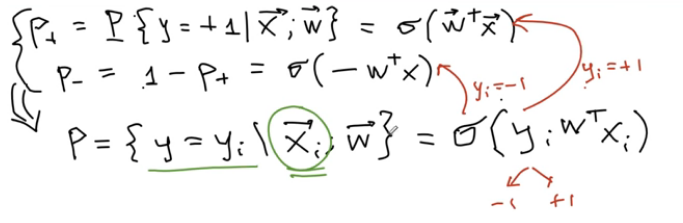
\includegraphics[width=0.65\linewidth]{mlcourse25}
\end{center}

\end{frame}

%%%%%%%%%%%%%%%%%%%%%%%%%%%%%%%%%%%%%%%%%%%%%%%%%%%%%%%%%%%%%%%%%%%%%%%%
\begin{frame}[fragile]\frametitle{Maximum Likelihood Estimation (MLE) Intuition}
\begin{itemize}
\item MLE Probability can be expressed as $P(y|x) = \Pi_{i=1}^l P(y = y_i | x_i)$, where $l$ are number of rows and $d$ columns/features.
\item Assumption: All observations (say, $(x1,y_1),(x_2,y_z) \ldots $ ) are IID (Independently Identically Distributed) data.
\item The probability can be equated in terms of Sigmoid, as seen before.
$= \Pi_{i=1}^l \sigma(y_i W^TX-i)$. We will maximize this. 
\item Instead of maximizing product, its better to maximize sum. so we take logs, then it becomes a sum, them maximize it. (Note: 'log' being monotonic,does not affect maximization)
\end{itemize}


\begin{center}
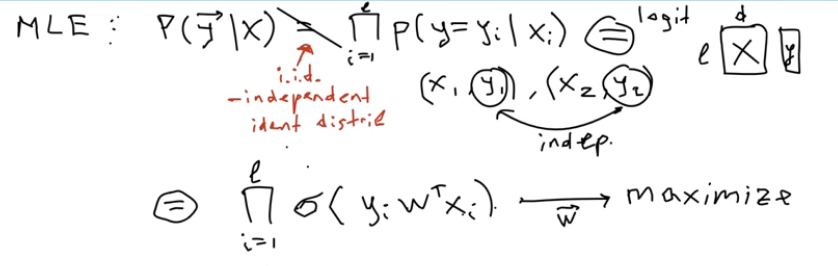
\includegraphics[width=0.6\linewidth]{mlcourse26}
\end{center}

\end{frame}


%%%%%%%%%%%%%%%%%%%%%%%%%%%%%%%%%%%%%%%%%%%%%%%%%%%%%%%%%%%%%%%%%%%%%%%%
\begin{frame}[fragile]\frametitle{Maximum Likelihood Estimation and Logistic Regression}
 \begin{itemize}

\item Let's see how an optimization problem for logistic regression is obtained from the MLE, namely, minimization of the logistic loss function. 
\item We have just seen that logistic regression models the probability of assigning an example to the class "+" as: $p_+(\textbf{x}_\text{i}) = P\left(y_i = 1 \mid \textbf{x}_\text{i}, \textbf{w}\right) = \sigma(\textbf{w}^T\textbf{x}_\text{i})$
\item Then, for the class "-", the corresponding expression is as follows:
$p_-(\textbf{x}_\text{i})  = P\left(y_i = -1 \mid \textbf{x}_\text{i}, \textbf{w}\right)  = 1 - \sigma(\textbf{w}^T\textbf{x}_\text{i}) = \sigma(-\textbf{w}^T\textbf{x}_\text{i})$

\item Both of these expressions can be cleverly combined into one (watch carefully, maybe you are being tricked): $P\left(y = y_i \mid \textbf{x}_\text{i}, \textbf{w}\right) = \sigma(y_i\textbf{w}^T\textbf{x}_\text{i})$
\end{itemize}

\end{frame}

%%%%%%%%%%%%%%%%%%%%%%%%%%%%%%%%%%%%%%%%%%%%%%%%%%%%%%%%%%%%%%%%%%%%%%%%
\begin{frame}[fragile]\frametitle{Geometrical Interpretation}
 \begin{itemize}

\item It is known (or given or assumed!!) find the distance from the point with a radius-vector $x_A$ to a plane defined by the equation $\textbf{w}^\text{T}\textbf{x} = 0$

\item Answer: $\rho(\textbf{x}_A, \textbf{w}^\text{T}\textbf{x} = 0) = \frac{\textbf{w}^\text{T}\textbf{x}_A}{||\textbf{w}||}$


\begin{center}
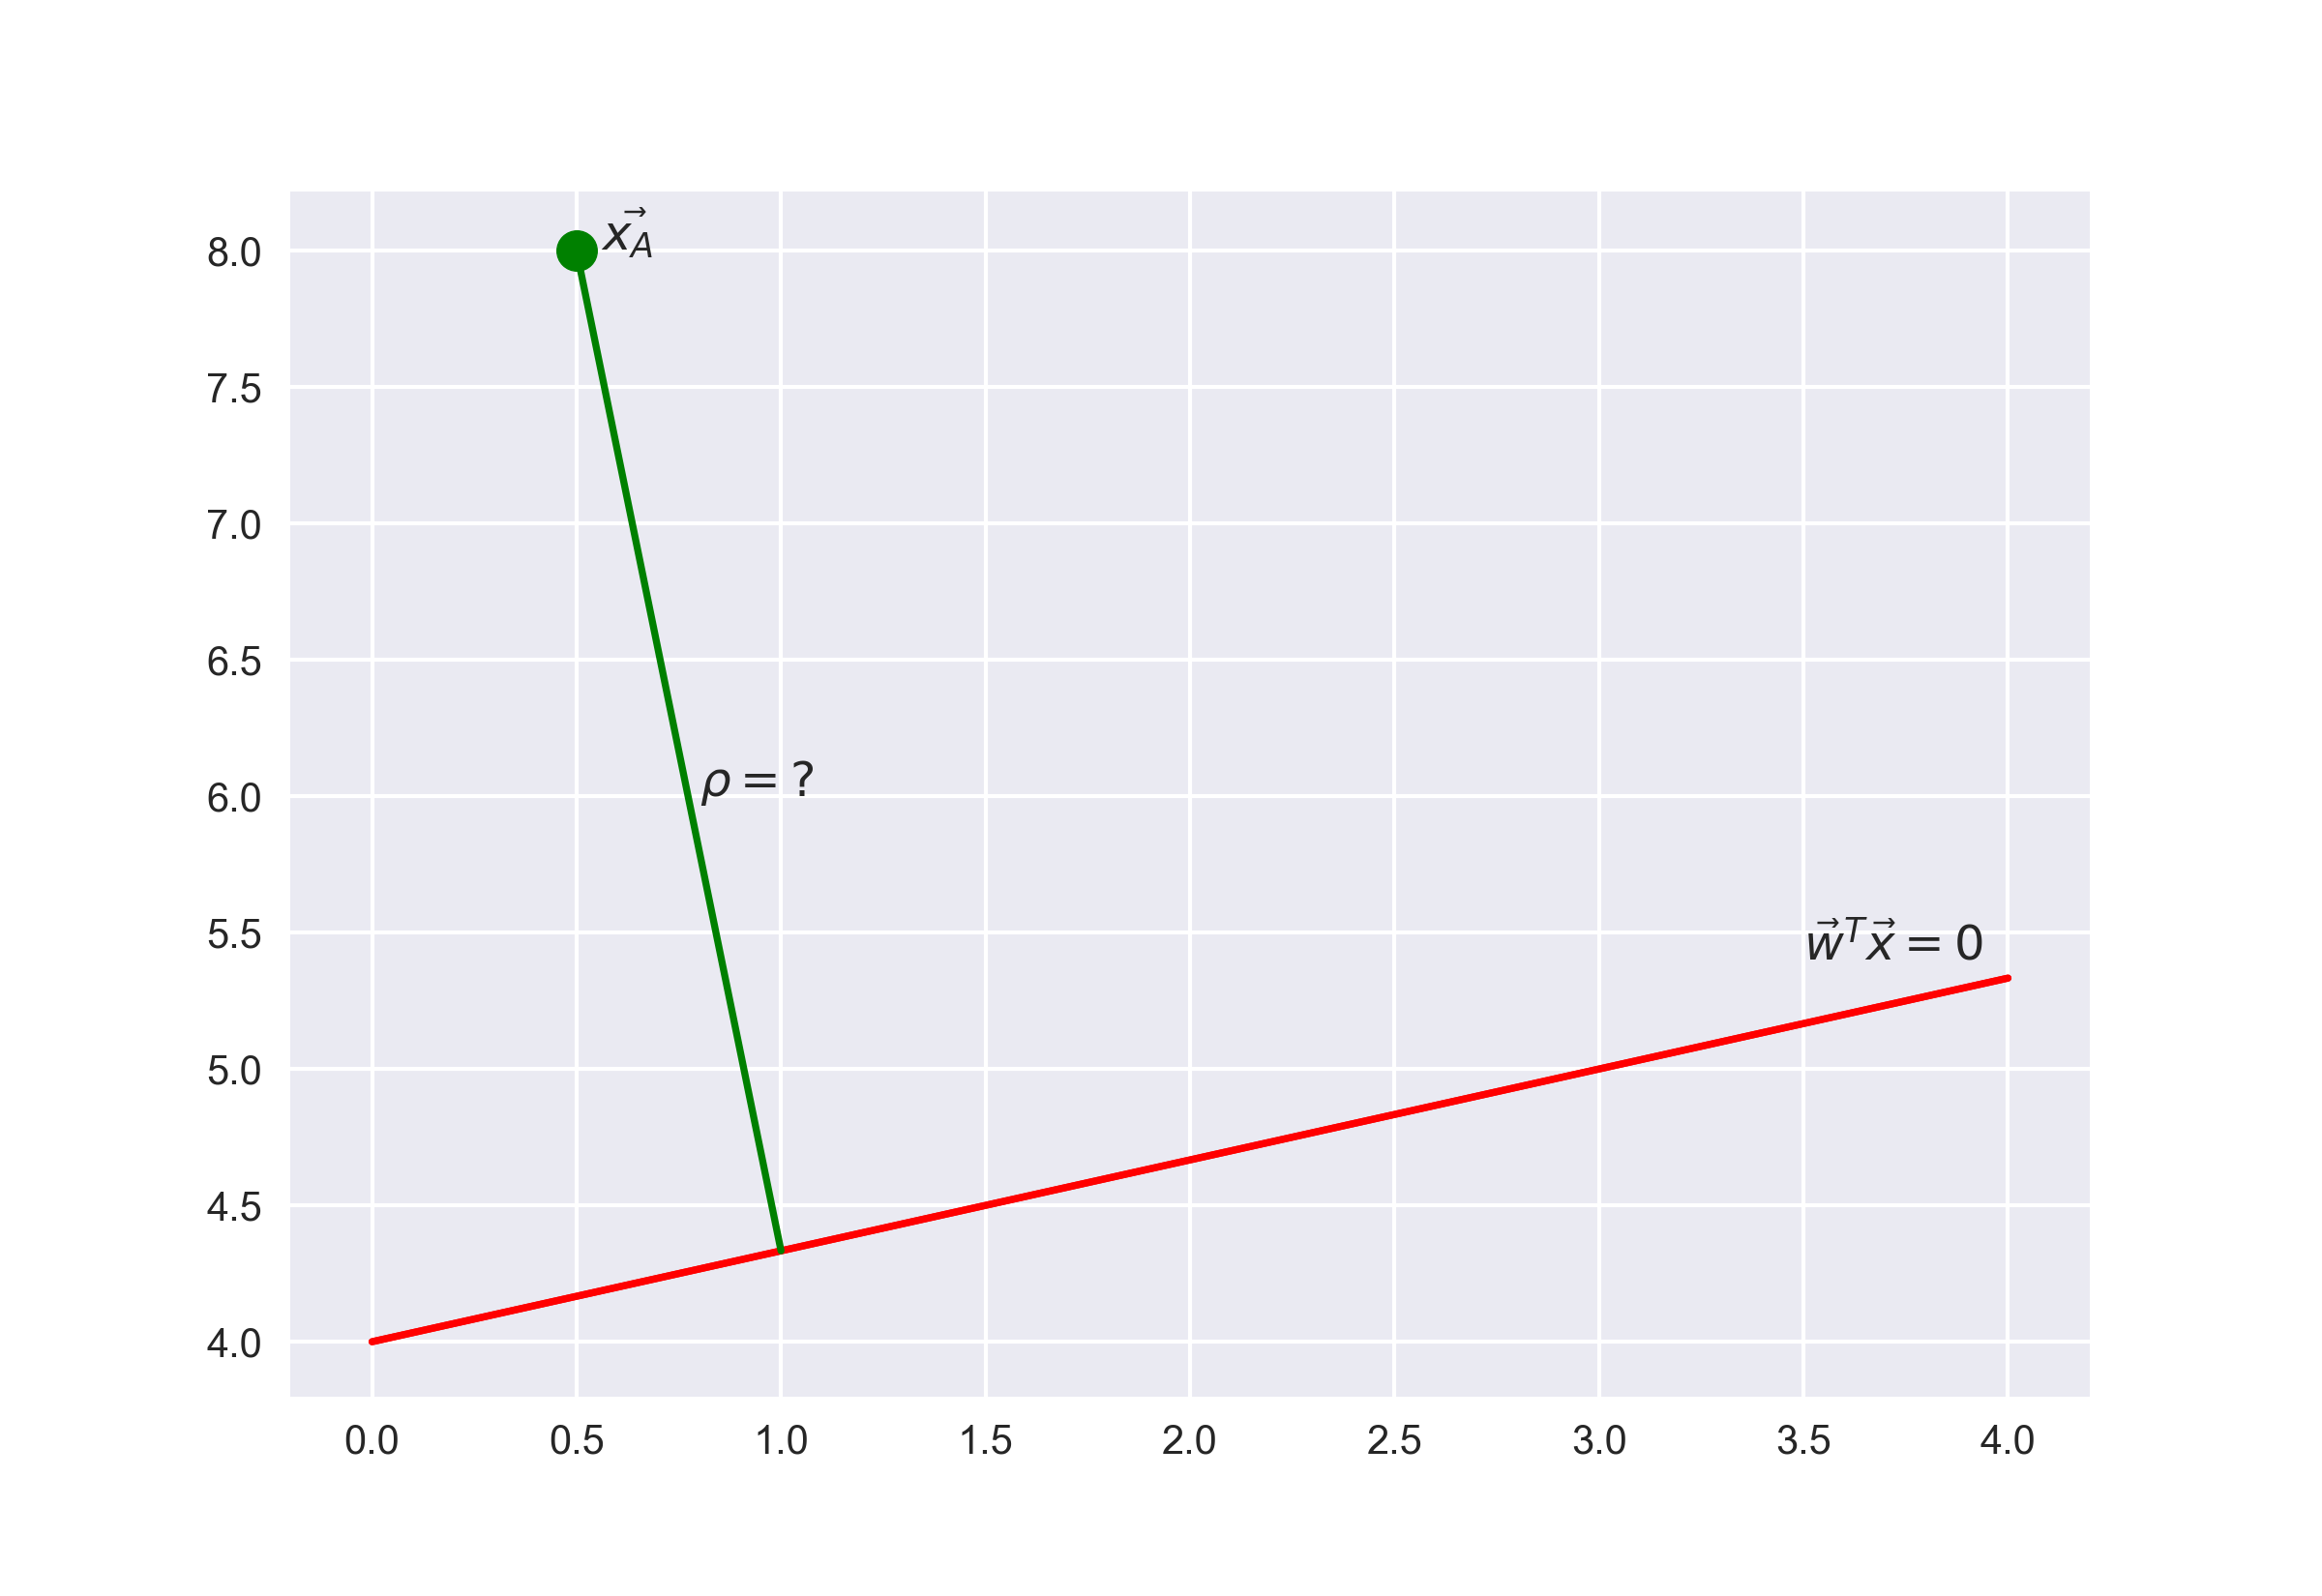
\includegraphics[width=0.45\linewidth]{mlcourse21}
\end{center}

\item The greater the absolute value of the expression $\textbf{w}^\text{T}\textbf{x}_\text{i}$, the farther the point $x_i$ is from the plane $\textbf{w}^\text{T}\textbf{x} = 0$
\end{itemize}

\end{frame}


%%%%%%%%%%%%%%%%%%%%%%%%%%%%%%%%%%%%%%%%%%%%%%%%%%%%%%%%%%%%%%%%%%%%%%%%
\begin{frame}[fragile]\frametitle{Maximum Likelihood Estimation and Logistic Regression}
Trick:
 \begin{itemize}

\item In the expression $M(\textbf{x}_\text{i}) = y_i\textbf{w}^T\textbf{x}_\text{i}$, the $\textbf{w}^T\textbf{x}_\text{i}$ part is for the distance of $x$ from the hyperplane, but if we multiply it by $y$ then it is known as the margin of classification on the object $x_i$ (not to be confused with a gap, which is also called margin, in the SVM context). 
\item If it is non-negative, the model is correct in choosing the class of the object $x_i$; if it is negative, then the object $x_i$ is misclassified. 
\item Note that the margin is defined for objects in the training set only where real target class labels $y_i$ are known.
\item In following figures, green is correct whereas red is not.
\end{itemize}

\end{frame}



%%%%%%%%%%%%%%%%%%%%%%%%%%%%%%%%%%%%%%%%%%%%%%%%%%%%%%%%%%%%%%%%%%%%%%%%
\begin{frame}[fragile]\frametitle{Maximum Likelihood Estimation and Logistic Regression}
Hence, our expression $M(\textbf{x}_\text{i}) = y_i\textbf{w}^\text{T}\textbf{x}_\text{i}$ is a kind of "confidence" in our model's classification of the object $x_i$:
 \begin{itemize}

\item If the margin is large (in absolute value) and positive, the class label is set correctly, and the object is far away from the separating hyperplane i.e. classified confidently. See Point x3 on the picture;

\begin{center}
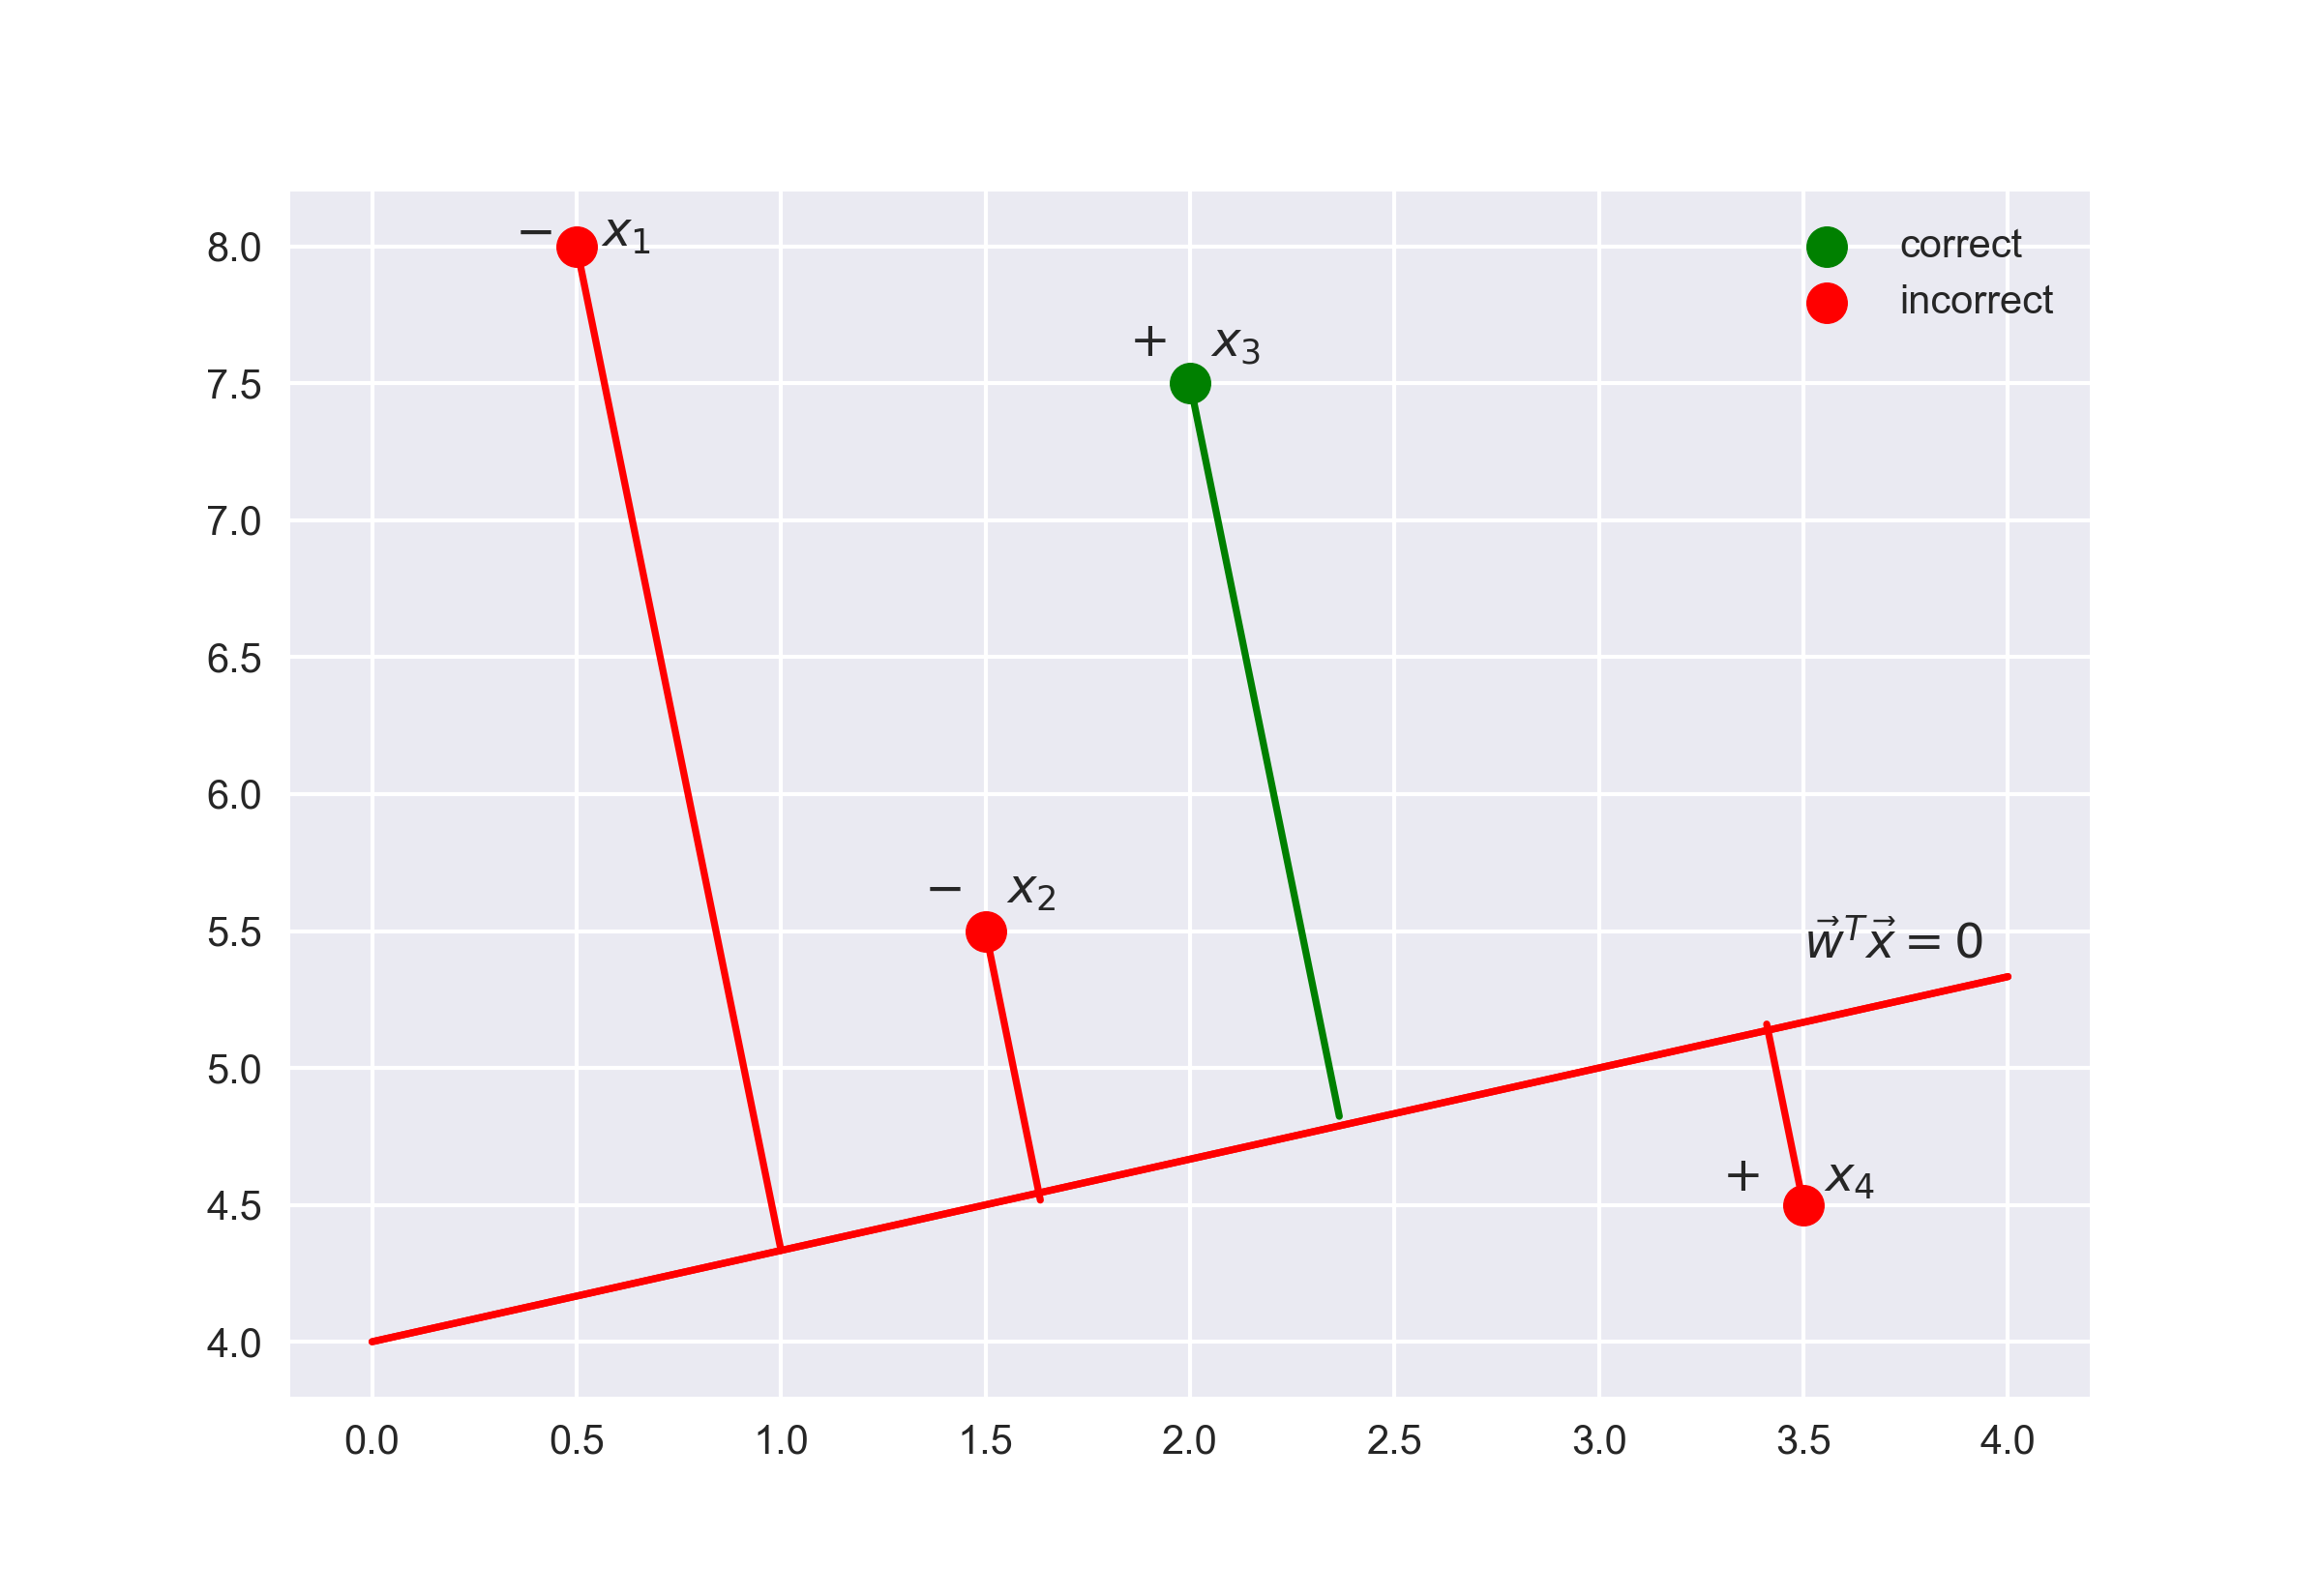
\includegraphics[width=0.45\linewidth]{mlcourse22}
\end{center}


\end{itemize}

\end{frame}


%%%%%%%%%%%%%%%%%%%%%%%%%%%%%%%%%%%%%%%%%%%%%%%%%%%%%%%%%%%%%%%%%%%%%%%%
\begin{frame}[fragile]\frametitle{Maximum Likelihood Estimation and Logistic Regression}
If the margin is large (in absolute value) and negative, then class label is set incorrectly, and the object is far from the separating hyperplane (the object is most likely an anomaly; for example, it could be improperly labeled in the training set). See Point $x_1$ on the picture;


\begin{center}
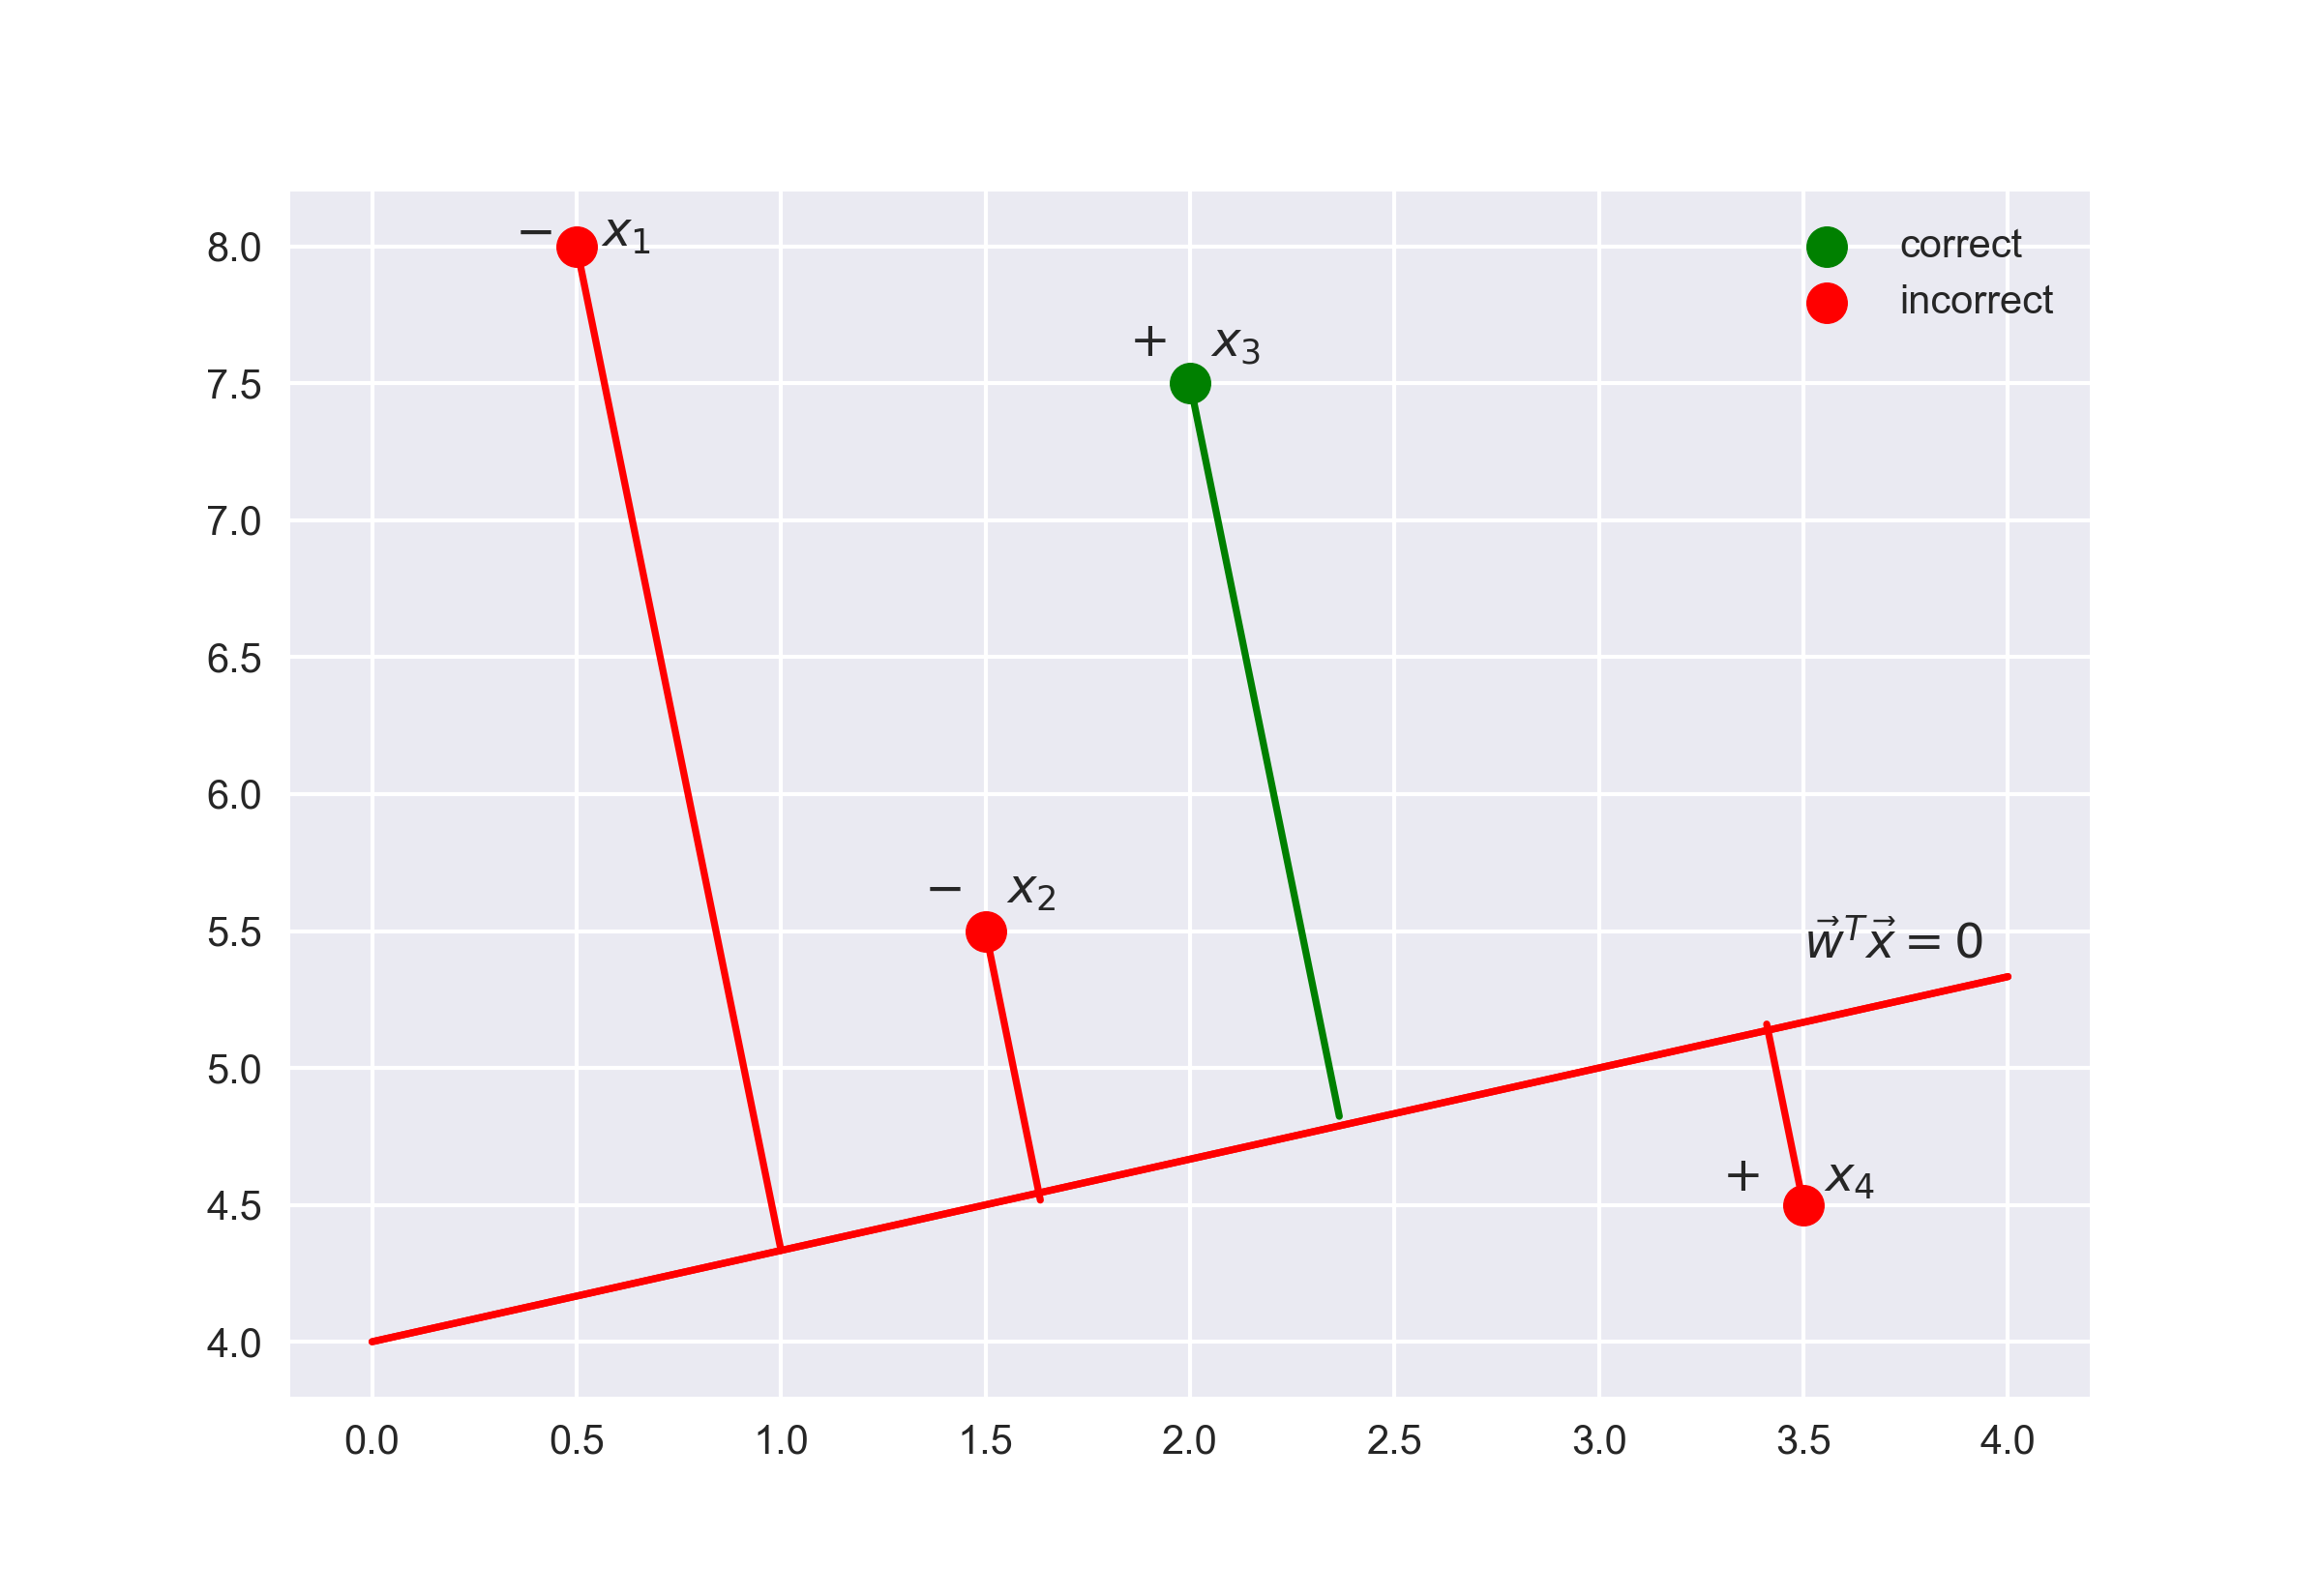
\includegraphics[width=0.45\linewidth]{mlcourse22}
\end{center}

\end{frame}


%%%%%%%%%%%%%%%%%%%%%%%%%%%%%%%%%%%%%%%%%%%%%%%%%%%%%%%%%%%%%%%%%%%%%%%%
\begin{frame}[fragile]\frametitle{Maximum Likelihood Estimation and Logistic Regression}

\begin{center}
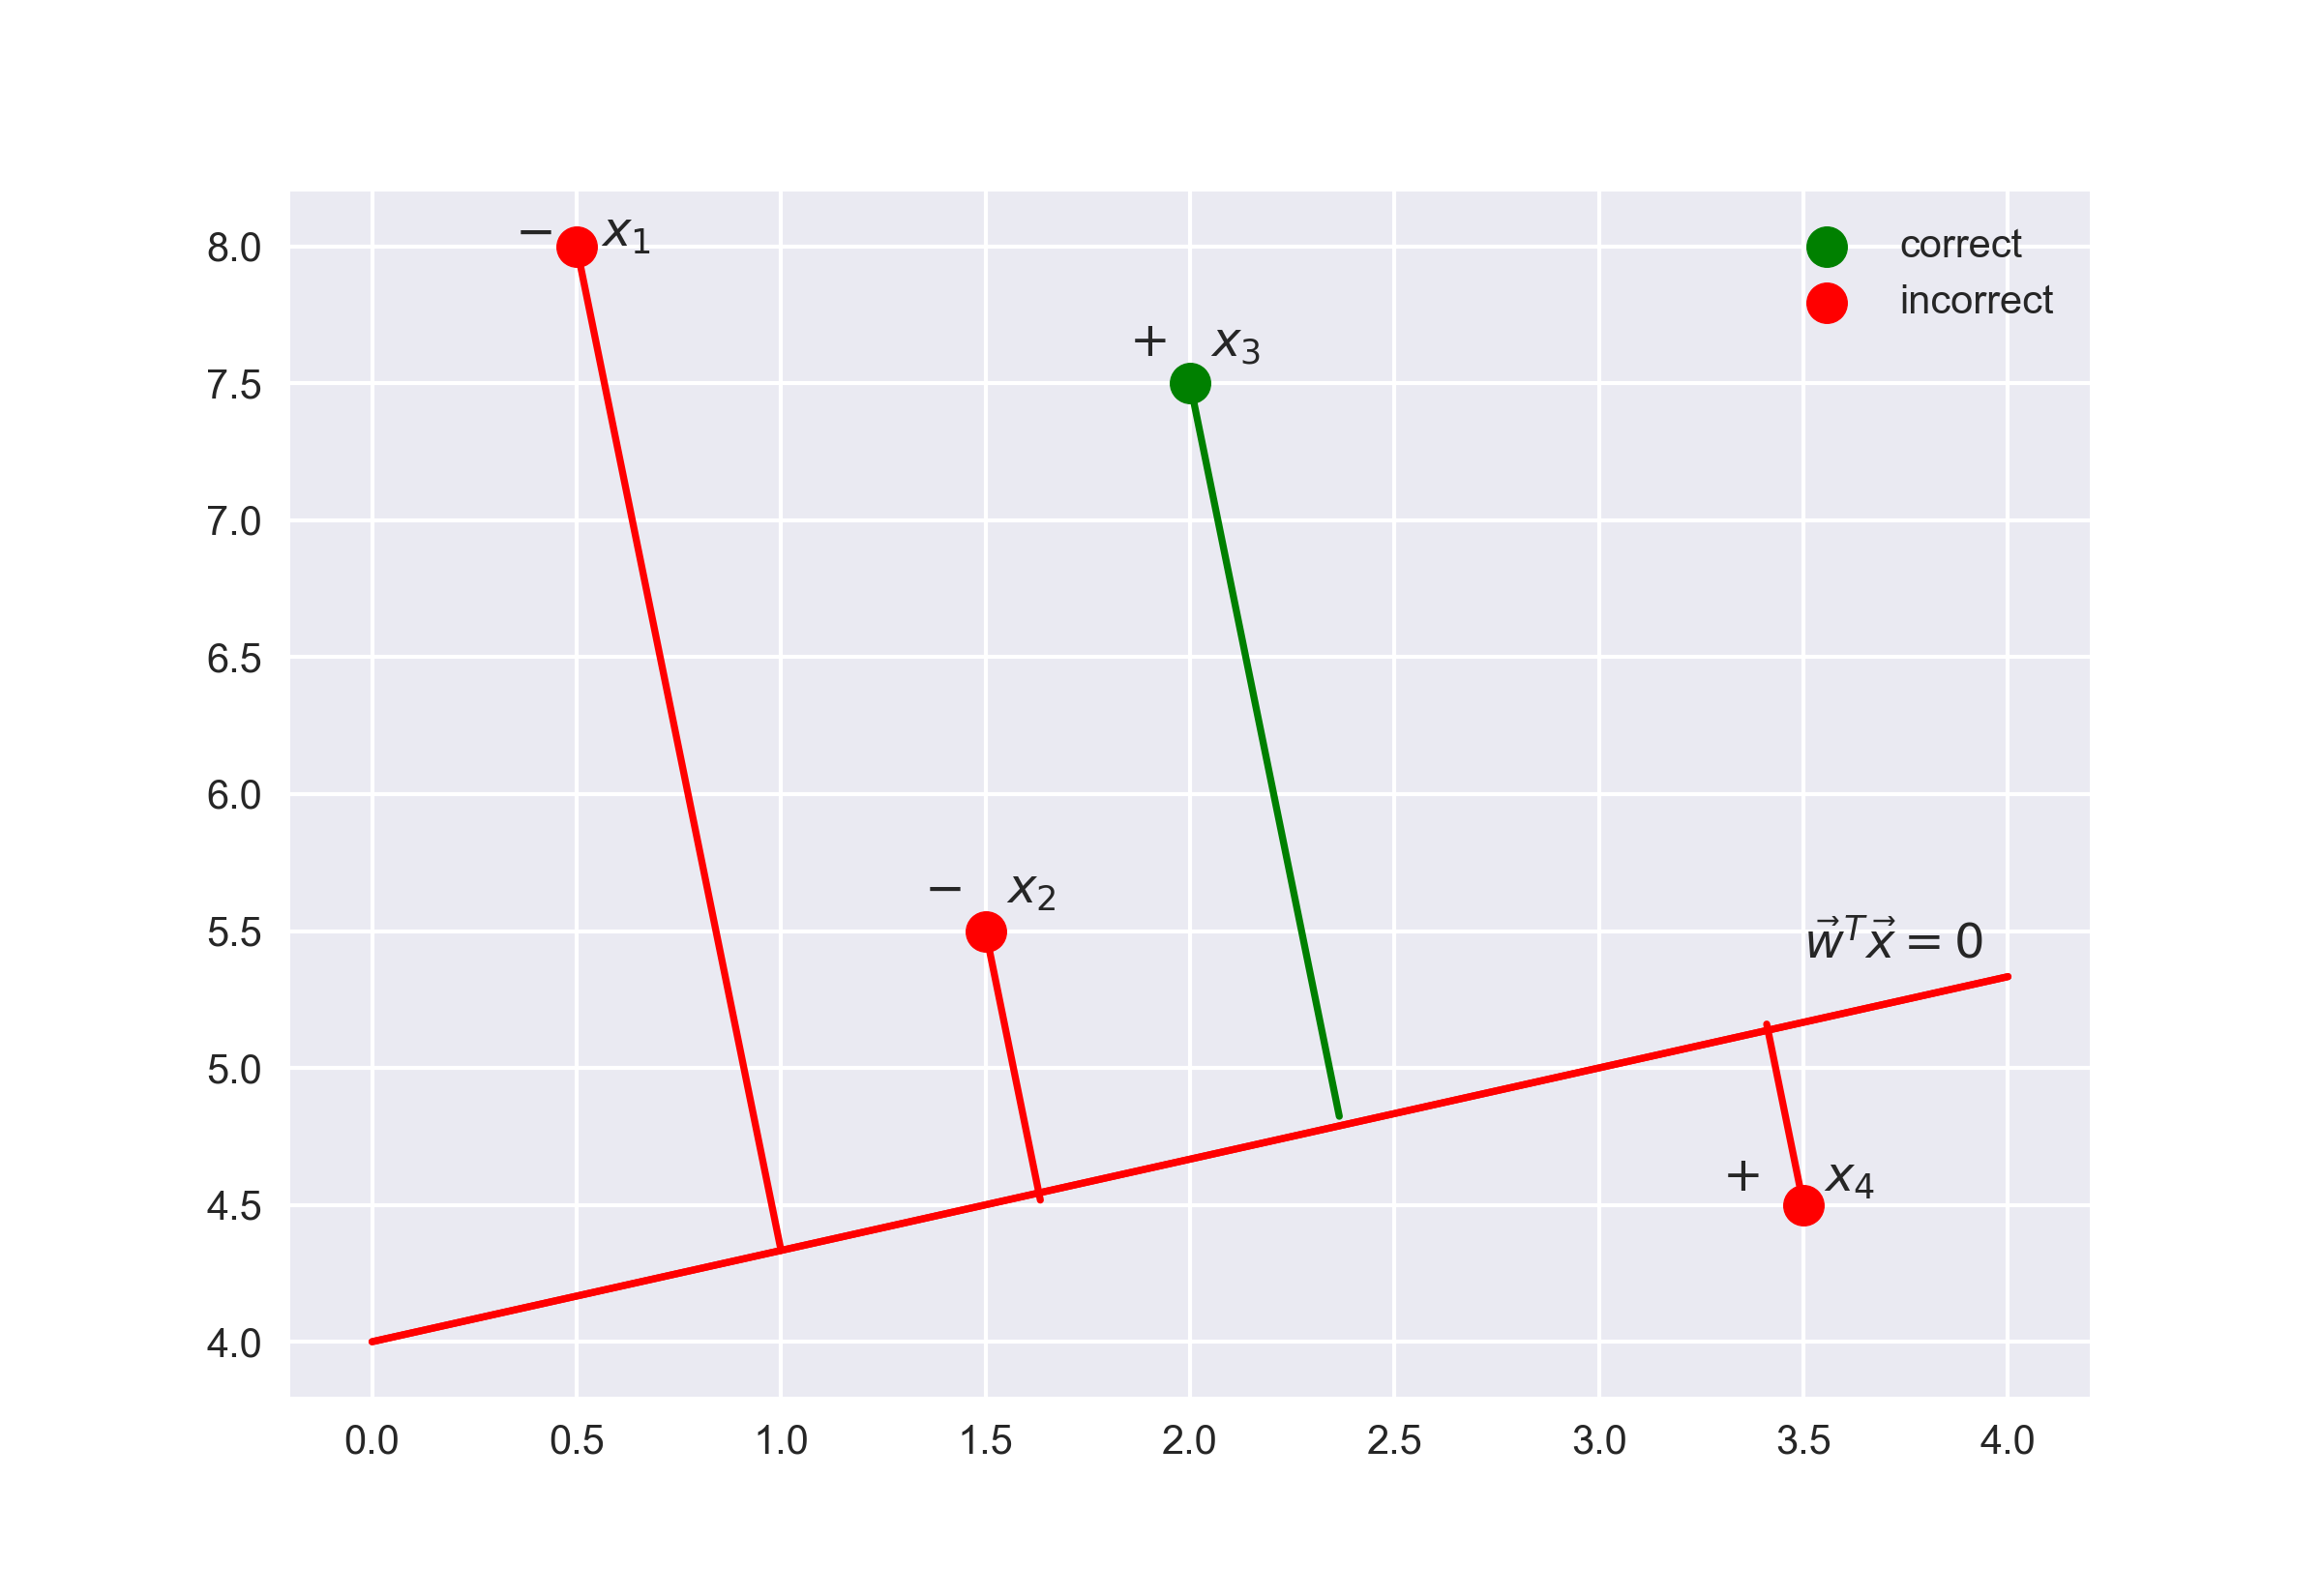
\includegraphics[width=0.45\linewidth]{mlcourse22}
\end{center}

If the margin is large (in absolute value) and negative, then class label is set incorrectly, and the object is far from the separating hyperplane (the object is most likely an anomaly; for example, it could be improperly labeled in the training set). See Point $x_1$ on the picture;


\end{frame}
%%%%%%%%%%%%%%%%%%%%%%%%%%%%%%%%%%%%%%%%%%%%%%%%%%%%%%%%%%%%%%%%%%%%%%%%
\begin{frame}[fragile]\frametitle{Maximum Likelihood Estimation and Logistic Regression}

\begin{center}
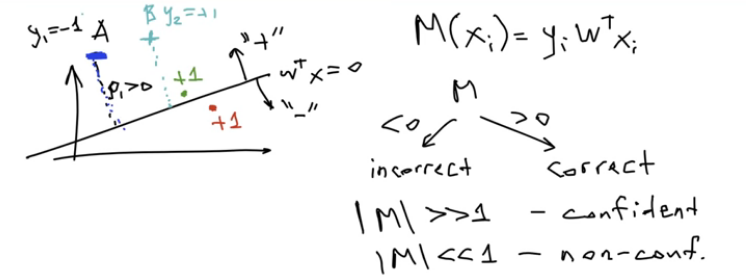
\includegraphics[width=0.8\linewidth]{mlcourse27}
\end{center}

We are now maximizing sigmoid of Margins wrt $W$, meaning a big sum of logs with exponential functions inside. We convert maximization to minimization with negative sign removed.

\begin{center}
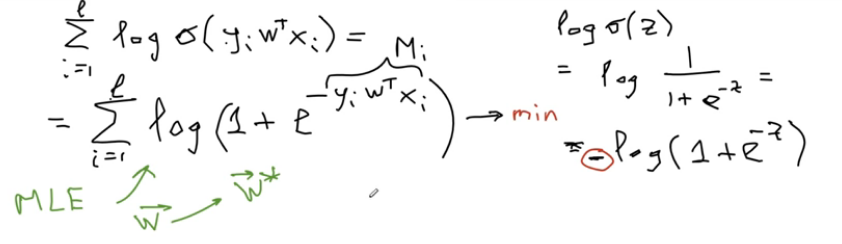
\includegraphics[width=0.8\linewidth]{mlcourse28}
\end{center}
This is Log Loss
\end{frame}

%%%%%%%%%%%%%%%%%%%%%%%%%%%%%%%%%%%%%%%%%%%%%%%%%%%%%%%%%%%%%%%%%%%%%%%%
\begin{frame}[fragile]\frametitle{Maximum Likelihood Estimation and Logistic Regression}
We use some Gradient Descent or something to get good $W$s.

\begin{center}
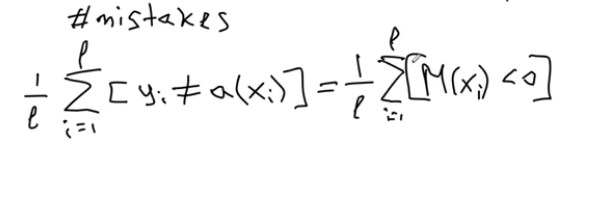
\includegraphics[width=0.8\linewidth]{mlcourse29}
\end{center}

% Evaluation: Number of cases where label does not agree with predictions. INcorrect are the ones with Margins negative.
% This is 1-0 Loss.
\end{frame}

%%%%%%%%%%%%%%%%%%%%%%%%%%%%%%%%%%%%%%%%%%%%%%%%%%%%%%%%%%%%%%%%%%%%%%%%
\begin{frame}[fragile]\frametitle{Maximum Likelihood Estimation and Logistic Regression}
 \begin{itemize}

 \item Let's now compute the likelihood of the data set i.e. the probability of observing the given vector y from data set X. We'll make a strong assumption: objects come independently from one distribution (i.i.d.). Then, we can write $P\left(\textbf{y} \mid \textbf{X}, \textbf{w}\right) = \prod_{i=1}^{\ell} P\left(y = y_i \mid \textbf{x}_\text{i}, \textbf{w}\right)$, where $\ell$ is the length of data set X (number of rows).
 
 \item As usual, let's take the logarithm of this expression because a sum is much easier to optimize than the product:
 
 $\log P\left(\textbf{y} \mid \textbf{X}, \textbf{w}\right) = \log \prod_{i=1}^{\ell} P\left(y = y_i \mid \textbf{x}_\text{i}, \textbf{w}\right) = \log \prod_{i=1}^{\ell} \sigma(y_i\textbf{w}^\text{T}\textbf{x}_\text{i})   =$
\end{itemize}

\end{frame}

%%%%%%%%%%%%%%%%%%%%%%%%%%%%%%%%%%%%%%%%%%%%%%%%%%%%%%%%%%%%%%%%%%%%%%%%
\begin{frame}[fragile]\frametitle{Maximum Likelihood Estimation and Logistic Regression}
 \begin{itemize}

 \item $  = \sum_{i=1}^{\ell} \log \sigma(y_i\textbf{w}^\text{T}\textbf{x}_\text{i}) = \sum_{i=1}^{\ell} \log \frac{1}{1 + \exp^{-y_i\textbf{w}^\text{T}\textbf{x}_\text{i}}} = - \sum_{i=1}^{\ell} \log (1 + \exp^{-y_i\textbf{w}^\text{T}\textbf{x}_\text{i}})$
 
 \item Maximizing the likelihood is equivalent to minimizing the expression: $\mathcal{L_{\log}} (\textbf X, \textbf{y}, \textbf{w}) = \sum_{i=1}^{\ell} \log (1 + \exp^{-y_i\textbf{w}^\text{T}\textbf{x}_\text{i}})$
 
 \item This is logistic loss function that is summed over all objects in the training set.
\end{itemize}

\end{frame}



%%%%%%%%%%%%%%%%%%%%%%%%%%%%%%%%%%%%%%%%%%%%%%%%%%%%%%%%%%%%%%%%%%%%%%%%
\begin{frame}[fragile]\frametitle{Maximum Likelihood Estimation and Logistic Regression}
 \begin{itemize}

 \item Let's look at the new function as a function of margin $L(M) = \log (1 + \exp^{-M})$ and plot it along with zero-one loss graph, which simply penalizes the model for error on each object by 1 (negative margin): $L_{1/0}(M) = [M < 0]$
 
 \begin{center}
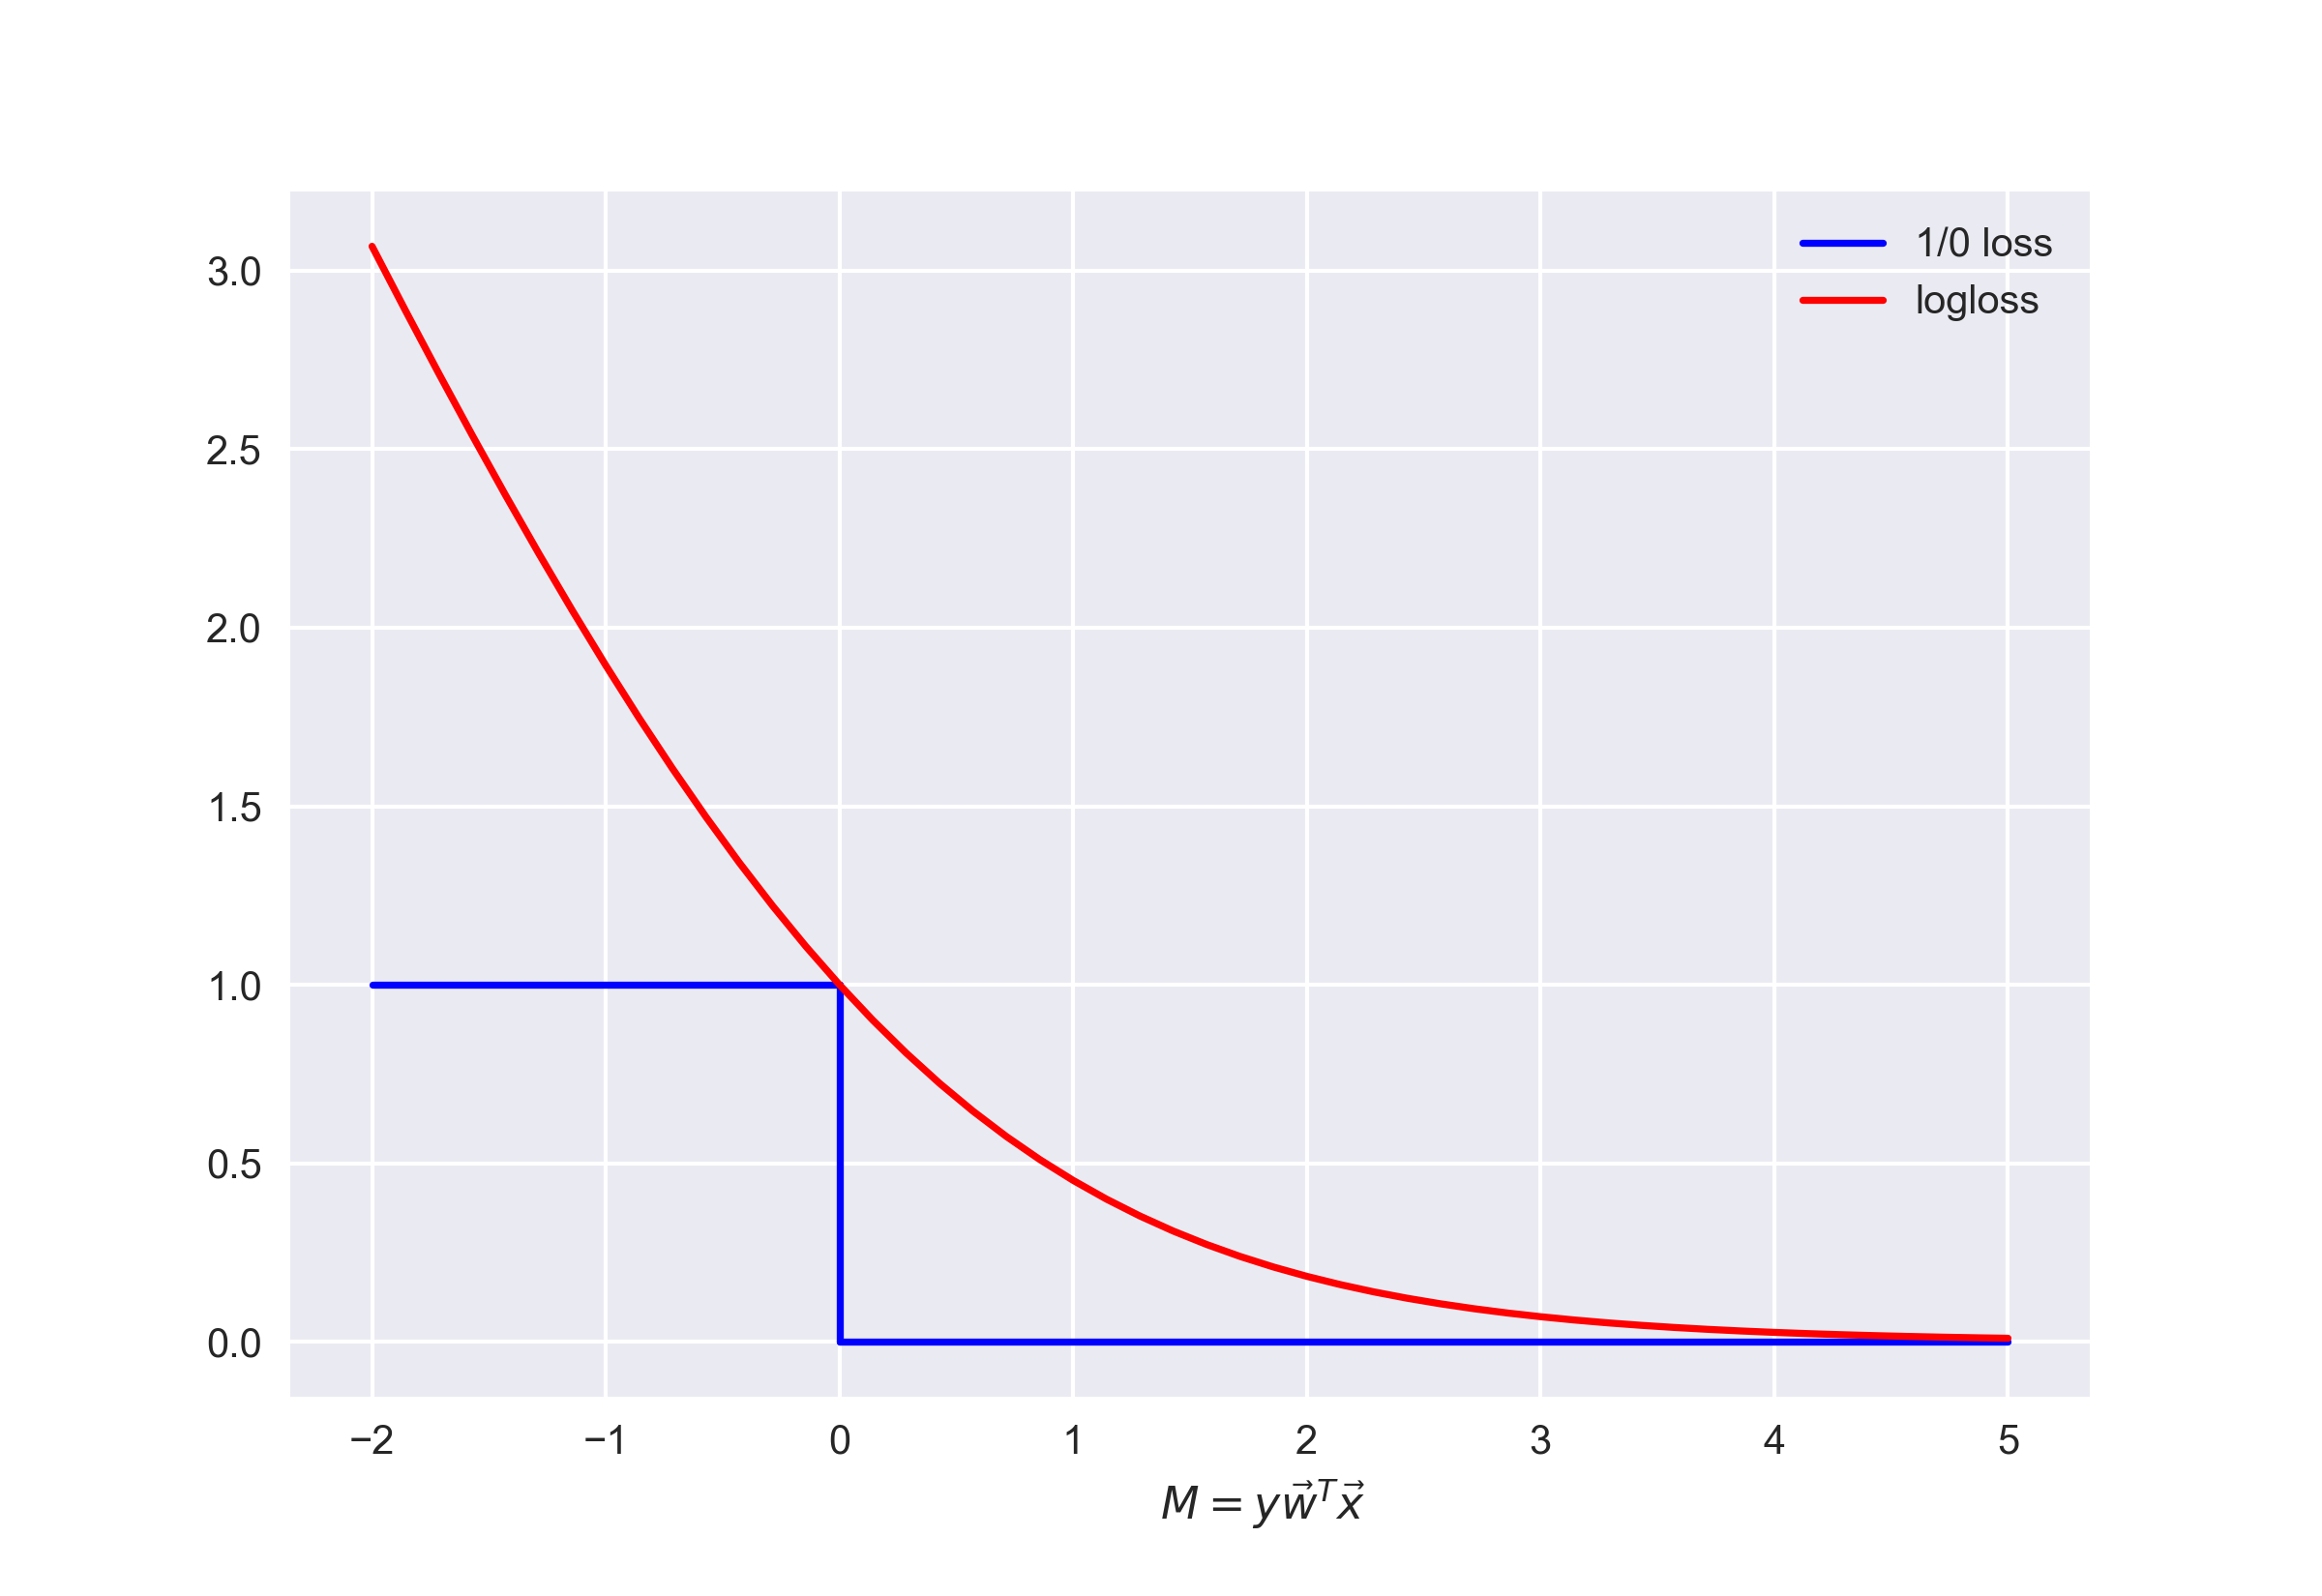
\includegraphics[width=0.4\linewidth]{mlcourse23}
\end{center}

\item The picture reflects the idea that, if we are not able to directly minimize the number of errors in the classification problem (at least not by gradient methods - derivative of the zero-one loss function at zero turns to infinity), we can minimize its upper bounds.
\end{itemize}

\end{frame}

%%%%%%%%%%%%%%%%%%%%%%%%%%%%%%%%%%%%%%%%%%%%%%%%%%%%%%%%%%%%%%%%%%%%%%%%
\begin{frame}[fragile]\frametitle{Maximum Likelihood Estimation and Logistic Regression}
 \begin{itemize}

 \item For the logistic loss function (where the logarithm is binary, but this does not matter), the following is valid: $\mathcal{L_{1/0}} (\textbf X, \textbf{y}, \textbf{w}) = \sum_{i=1}^{\ell} [M(\textbf{x}_\text{i}) < 0] \leq \sum_{i=1}^{\ell} \log (1 + \exp^{-y_i\textbf{w}^\text{T}\textbf{x}_\text{i}}) = \mathcal{L_{\log}} (\textbf X, \textbf{y}, \textbf{w}),$
 
 \item where $\mathcal{L_{1/0}} (\textbf X, \textbf{y})$ is simply the number of errors of logistic regression with weights w on a data set $(\textbf X, \textbf{y})$.
 
 \item Thus, by reducing the upper bound of $\mathcal{L_{log}}$ by the number of classification errors, we hope to reduce the number of errors itself.
\end{itemize}

\end{frame}



%%%%%%%%%%%%%%%%%%%%%%%%%%%%%%%%%%%%%%%%%%%%%%%%%%%%%%%%%%%%%%%%%%%%%%%%
\begin{frame}[fragile]\frametitle{LogLoss Defined}
Instead of Squared-Loss defined for Linear Regression, we have Log-Loss defined for Logistic Regression.
\begin{center}
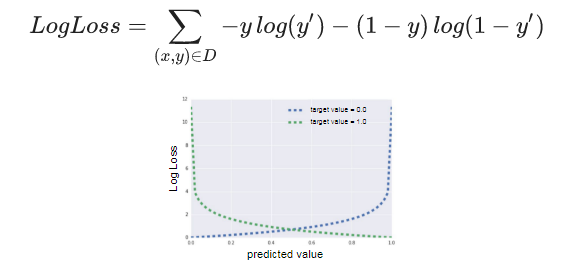
\includegraphics[width=0.8\linewidth]{logistic2}
\end{center}

Loss is most near 0 or 1. We are trying to minimize it.

%(Note: Looks very similar to Shannon's entropy measure, information theory)

% % (Ref: https://developers.google.com/machine-learning/crash-course/logistic-regression/video-lecture)
\end{frame}

%%%%%%%%%%%%%%%%%%%%%%%%%%%%%%%%%%%%%%%%%%%%%%%%%%%%%%%%%%%%%%%%%%%%%%%%
\begin{frame}[fragile]\frametitle{LogLoss Rational : Maximum Likelihood Estimation}
\begin{itemize}
\item For a survey on whether India will win the next world cup, 400 answered.
\item 117 people were Positive.
\item Then, it is reasonable to assume that the probability that the next respondent feels that India will win,  is $\frac{117}{400} \approx 29\%$
\item This intuitive assessment is not only good but also a maximum likelihood estimate.
\end{itemize}
\end{frame}

%%%%%%%%%%%%%%%%%%%%%%%%%%%%%%%%%%%%%%%%%%%%%%%%%%%%%%%%%%%%%%%%%%%%%%%%
\begin{frame}[fragile]\frametitle{Background: Bernoulli distribution}
\begin{itemize}
\item Bernoulli distribution: a random variable has a Bernoulli distribution if it takes only two values (1 and 0 with probability $\theta$ and $1- \theta$ respectively) and has the following probability distribution function: 

$ p \left( \theta, x\right) = \theta^{x} \left(1 - \theta\right)^{\left(1 - x\right)}, x \in \left\{0, 1\right\}$
\item This distribution is exactly what we need, and the distribution parameter $\theta$ is the estimate of the probability that a person feels India will win.
\end{itemize}
\end{frame}

%%%%%%%%%%%%%%%%%%%%%%%%%%%%%%%%%%%%%%%%%%%%%%%%%%%%%%%%%%%%%%%%%%%%%%%%
\begin{frame}[fragile]\frametitle{Background: Bernoulli distribution}
\begin{itemize}
\item In our 400 independent experiments, let's denote their outcomes as $\textbf{x} = \left(x_1, x_2, \ldots, x_{400}\right)$
\item Let's write down the likelihood of our data (observations), i.e. the probability of observing exactly these 117 realizations of the random variable $x=1$ and 283 realizations of $x=0$:
$ p(\textbf{x}; \theta) = \prod_{i=1}^{400} \theta^{x_i} \left(1 - \theta\right)^{\left(1 - x_i\right)} = \theta^{117} \left(1 - \theta\right)^{283}$
\end{itemize}
\end{frame}

%%%%%%%%%%%%%%%%%%%%%%%%%%%%%%%%%%%%%%%%%%%%%%%%%%%%%%%%%%%%%%%%%%%%%%%%
\begin{frame}[fragile]\frametitle{Background: Bernoulli distribution}
\begin{itemize}
\item Next, we will maximize the expression with respect to $\theta$. Most often this is not done with the likelihood $p(\textbf{x}; \theta)$ but with its logarithm (the monotonic transformation does not change the solution but simplifies calculation greatly):
$ \log p(\textbf{x}; \theta) = \log \prod_{i=1}^{400} \theta^{x_i} \left(1 - \theta\right)^{\left(1 - x_i\right)} =$

$ = \log \theta^{117} \left(1 - \theta\right)^{283} =  117 \log \theta + 283 \log \left(1 - \theta\right)$
\item Now, we want to find such a value of $\theta$ that will maximize the likelihood.
\end{itemize}
\end{frame}

%%%%%%%%%%%%%%%%%%%%%%%%%%%%%%%%%%%%%%%%%%%%%%%%%%%%%%%%%%%%%%%%%%%%%%%%
\begin{frame}[fragile]\frametitle{Background: Bernoulli distribution}
\begin{itemize}
\item For this purpose, we'll take the derivative with respect to $\theta$, set it to zero, and solve the resulting equation: $\Large  \frac{\partial \log p(\textbf{x}; \theta)}{\partial \theta} = \frac{\partial}{\partial \theta} \left(117 \log \theta + 283 \log \left(1 - \theta\right)\right) = \frac{117}{\theta} - \frac{283}{1 - \theta};$

\item It turns out that our intuitive assessment is exactly the maximum likelihood estimate.
\end{itemize}
\end{frame}

%%%%%%%%%%%%%%%%%%%%%%%%%%%%%%%%%%%%%%%%%%%%%%%%%%%%%%%%%%%%%%%%%%%%%%%%
\begin{frame}[fragile]\frametitle{Cost function of logistic regression}
\begin{itemize}
\item We have a dataset X consisting of m data-points and n features. And there is a class variable y a vector of length m which can have two values 1 or 0.
\item  Now logistic regression says that the probability that class variable value yi=1 , i=1,2,...m can be modeled as follows:
$P( y_i =1 | \mathbf{x}_i ; \theta) = h_{\theta}(\mathbf{x}_i) = \dfrac{1}{1+e^{(- \theta^T \mathbf{x}_i)}}$
\item So $y_i = 1$ with probability $h_{\theta}(\mathbf{x}_i)$ and $y_i=0$ with probability $1-h_{\theta}(\mathbf{x}_i)$.
\end{itemize}

{\tiny (Ref: Deriving cost function using MLE :Why use log function? - Stack Overflow)}
\end{frame}

%%%%%%%%%%%%%%%%%%%%%%%%%%%%%%%%%%%%%%%%%%%%%%%%%%%%%%%%%%%%%%%%%%%%%%%%
\begin{frame}[fragile]\frametitle{Cost function of logistic regression}
\begin{itemize}
\item This can be combined into a single equation as follows, ( actually $y_i$ follows a Bernoulli distribution)
$P(y_i ) = h_{\theta}(\mathbf{x}_i)^{y_i} (1 - h_{\theta}(\mathbf{x}_i))^{1-y_i}$
\item $P(y_i)$ is known as the likelihood of single data point $x_i$, i.e. given the value of $y_i$ what is the probability of $x_i$ occurring. it is the conditional probability $P(\mathbf{x}_i | y_i)$.
\item The likelihood of the entire dataset X is the product of the individual data point likelihoods. Thus

$P(\mathbf{X}|\mathbf{y}) = \prod_{i=1}^{m} P(\mathbf{x}_i | y_i) = \prod_{i=1}^{m} h_{\theta}(\mathbf{x}_i)^{y_i} (1 - h_{\theta}(\mathbf{x}_i))^{1-y_i}$
\end{itemize}

{\tiny (Ref: Deriving cost function using MLE :Why use log function? - Stack Overflow)}
\end{frame}

%%%%%%%%%%%%%%%%%%%%%%%%%%%%%%%%%%%%%%%%%%%%%%%%%%%%%%%%%%%%%%%%%%%%%%%%
\begin{frame}[fragile]\frametitle{Cost function of logistic regression}
\begin{itemize}
\item Now the principle of maximum likelihood says that we find the parameters that maximise likelihood $P(\mathbf{X}|\mathbf{y})$.
\item logarithms are used because they convert products into sums and do not alter the maximization search, as they are monotone increasing functions. Here too we have a product form in the likelihood.So we take the natural logarithm as maximising the likelihood is same as maximising the log likelihood, so log likelihood $L(\theta)$ is now:

$L(\theta) = \log(P(\mathbf{X}|\mathbf{y}) =  \sum_{i=1}^{m} y_i \log(h_{\theta}(\mathbf{x}_i)) + (1-y_i) \log(1 - h_{\theta}(\mathbf{x}_i))$
\end{itemize}

{\tiny (Ref: Deriving cost function using MLE :Why use log function? - Stack Overflow)}
\end{frame}

%%%%%%%%%%%%%%%%%%%%%%%%%%%%%%%%%%%%%%%%%%%%%%%%%%%%%%%%%%%%%%%%%%%%%%%%
\begin{frame}[fragile]\frametitle{Cost function of logistic regression}
\begin{itemize}
\item Since in linear regression we found the $\theta$ that minimizes our cost function , here too for the sake of consistency, we would like to have a minimization problem. And we want the average cost over all the data points. 
\item Currently, we have a maximization of $L(\theta)$. Maximization of $L(\theta)$ is equivalent to minimization of $-L(\theta)$. And using the average cost over all data points, our cost function for logistic regression comes out to be, $J(\theta) = - \dfrac{1}{m} L(\theta)$

$= - \dfrac{1}{m} \left(  \sum_{i=1}^{m} y_i \log (h_{\theta}(\mathbf{x}_i)) +  (1-y_i) \log (1 - h_{\theta}(\mathbf{x}_i)) \right )$
\end{itemize}

{\tiny (Ref: Deriving cost function using MLE :Why use log function? - Stack Overflow)}
\end{frame}

%%%%%%%%%%%%%%%%%%%%%%%%%%%%%%%%%%%%%%%%%%%%%%%%%%%%%%%%%%%%%%%%%%%%%%%%
\begin{frame}[fragile]\frametitle{Cost function of logistic regression}
\begin{itemize}
\item Now we can also understand why the cost for single data point comes as follows:
\item the cost for a single data point is $=  -\log( P(\mathbf{x}_i | y_i))$ which can be written as $- \left ( y_i \log (h_{\theta}(\mathbf{x}_i)) + (1 - y_i) \log (1 - h_{\theta}(\mathbf{x}_i) \right )$
\item We can now split the above into two depending upon the value of $y_i$. Thus we get $J(h_{\theta}(\mathbf{x}_i), y_i) = - \log (h_{\theta}(\mathbf{x}_i))  , \text{     if } y_i=1$ and
$ J(h_{\theta}(\mathbf{x}_i), y_i) = - \log (1 -  (h_{\theta}(\mathbf{x}_i) )  , \text{    if } y_i=0$
\end{itemize}

{\tiny (Ref: Deriving cost function using MLE :Why use log function? - Stack Overflow)}
\end{frame}



%%%%%%%%%%%%%%%%%%%%%%%%%%%%%%%%%%%%%%%%%%%%%%%%%%%%%%%%%%%%%%%%%%%%%%%%%%%%%%%%%
\begin{frame}[fragile]\frametitle{}
\begin{center}
{\Large Evaluation Metrics}
\end{center}
\end{frame}


%%%%%%%%%%%%%%%%%%%%%%%%%%%%%%%%%%%%%%%%%%%%%%%%%%%%%%%%%%%%%%%%%%%%%%%%
\begin{frame}[fragile]\frametitle{Accuracy}
\begin{itemize}
\item How do we evaluate classification models?
\item One possible measure: Accuracy
	\begin{itemize}
	\item the fraction of predictions we got right
	\end{itemize}
\item Accuracy Can Be Misleading
	% \begin{itemize}
	% \item Most often when different kinds of mistakes have different costs
	% \item Typical case includes class imbalance, when positives or negatives are extremely rare
	% \end{itemize}
\end{itemize}

% (Ref: https://developers.google.com/machine-learning/crash-course/classification/video-lecture)
\end{frame}

%%%%%%%%%%%%%%%%%%%%%%%%%%%%%%%%%%%%%%%%%%%%%%%%%%%%%%%%%%%%%%%%%%%%%%%%
\begin{frame}[fragile]\frametitle{Accuracy}
\begin{itemize}
\item In case of cancer dataset, if you blatantly predict ``No Cancer'' you are going to be right 99\% times, as thats the percent of Non-Cancer patients in the population.
\item In this case, such great accuracy is actually useless, as the class/target is imbalanced. 
\item Need Confusion Matrix.
\end{itemize}

% (Ref: https://developers.google.com/machine-learning/crash-course/classification/video-lecture)
\end{frame}


%%%%%%%%%%%%%%%%%%%%%%%%%%%%%%%%%%%%%%%%%%%%%%%%%%%%%%%%%%%%%%%%%%%%%%%%
\begin{frame}[fragile]\frametitle{What is ROC?}

\begin{columns}
\begin{column}[T]{0.5\linewidth}
\begin{itemize}
\item ROC : Receiver Operating Characteristics Curve
\item ROC tells us about how good
the model can distinguish between two things (e.g If a patient has a
disease or no). 
\item Better models can accurately distinguish between the two.
\item Predictions are plotted on x, and colors show True or false. Y is frequency or counts.
\end{itemize}
\end{column}
\begin{column}[T]{0.5\linewidth}

\begin{center}
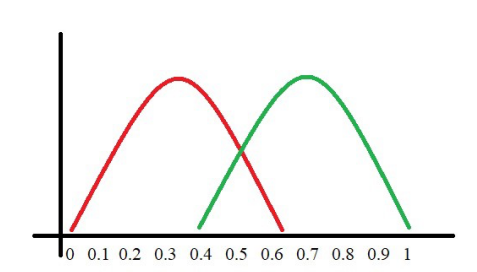
\includegraphics[width=0.9\linewidth]{roc1}
\end{center}

\tiny{(Ref: Let's learn about AUC ROC Curve! – GreyAtom)}
\end{column}

\end{columns}
\end{frame}

%%%%%%%%%%%%%%%%%%%%%%%%%%%%%%%%%%%%%%%%%%%%%%%%%%%%%%%%%%%%%%%%%%%%%%%%
\begin{frame}[fragile]\frametitle{What is ROC?}

\begin{columns}
\begin{column}[T]{0.5\linewidth}
\begin{itemize}
\item Pick a value where we need to set the cut off say, “0.5” as shown
\item All the positive values above the threshold will be “True Positives”
\item Negative values above the threshold will be “False Positives” as they
are predicted incorrectly as positives.
\item All the negative values below the threshold will be “True Negatives”
\item Positive values below the threshold will be “False Negative” as they
are predicted incorrectly as negatives.
\end{itemize}
\end{column}
\begin{column}[T]{0.5\linewidth}

\begin{center}
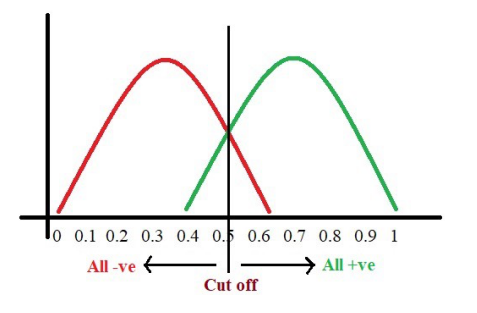
\includegraphics[width=0.9\linewidth]{roc2}

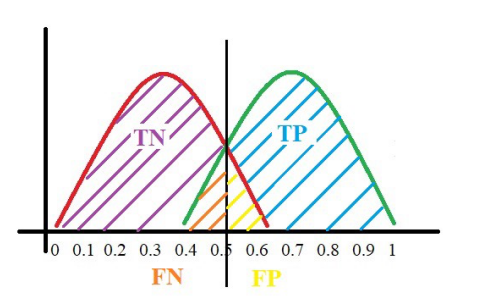
\includegraphics[width=0.9\linewidth]{roc3}
\end{center}

\tiny{(Ref: Let's learn about AUC ROC Curve! – GreyAtom)}
\end{column}

\end{columns}
\end{frame}

%%%%%%%%%%%%%%%%%%%%%%%%%%%%%%%%%%%%%%%%%%%%%%%%%%%%%%%%%%%%%%%%%%%%%%%%
\begin{frame}[fragile]\frametitle{What is Sensitivity and Speci4city?}

\begin{columns}
\begin{column}[T]{0.5\linewidth}
\begin{itemize}
\item Sensitivity or Recall = TP/TP + FN.
\item Specificity = TN/TN + FP.
\item When we decrease the threshold, we get more positive values thus
increasing the sensitivity. Meanwhile, this will decrease the specificity.
\item and vice versa. Meaning, there is a trade-off.
\item  Instead
of Specificity we use (1 - Specificity) and the graph will look something
like the bottom one:
\end{itemize}
\end{column}
\begin{column}[T]{0.5\linewidth}

\begin{center}
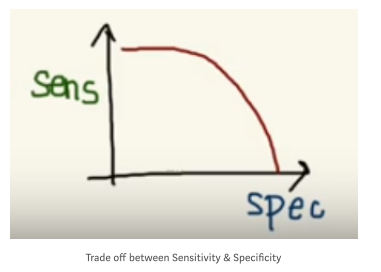
\includegraphics[width=0.8\linewidth]{roc4}

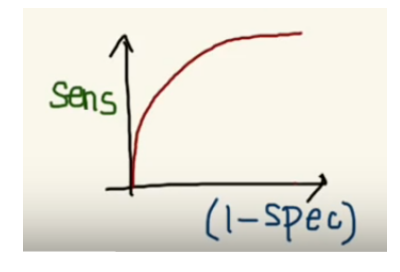
\includegraphics[width=0.8\linewidth]{roc5}
\end{center}

\tiny{(Ref: Let's learn about AUC ROC Curve! – GreyAtom)}
\end{column}

\end{columns}
\end{frame}

%%%%%%%%%%%%%%%%%%%%%%%%%%%%%%%%%%%%%%%%%%%%%%%%%%%%%%%%%%%%%%%%%%%%%%%%
\begin{frame}[fragile]\frametitle{Why do we use (1- Specificity)?}

\begin{columns}
\begin{column}[T]{0.5\linewidth}
\begin{itemize}
\item Let’s derive what exactly is (1-Specificity)
\item  Specificity gives us the True Negative Rate
\item  (1 - Specificity) gives us the  False Positive Rate Rate
\item So now we are just looking at the positives. 
\item As we increase the threshold,
we decrease the TPR as well as the FPR and when we decrease the
threshold, we are increasing the TPR and FPR.
\end{itemize}
\end{column}
\begin{column}[T]{0.5\linewidth}

\begin{center}
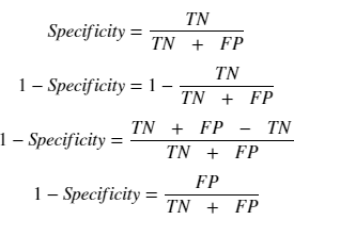
\includegraphics[width=0.8\linewidth]{roc7}
\end{center}

\tiny{(Ref: Let's learn about AUC ROC Curve! – GreyAtom)}
\end{column}

\end{columns}
\end{frame}


%%%%%%%%%%%%%%%%%%%%%%%%%%%%%%%%%%%%%%%%%%%%%%%%%%%%%%%%%%%%%%%%%%%%%%%%
\begin{frame}[fragile]\frametitle{What is AUC?}

\begin{columns}
\begin{column}[T]{0.5\linewidth}
\begin{itemize}
\item The AUC is the area under the ROC curve. 
\item It gives us a good idea
of how well the model performances.
\item AUC ROC indicates how well the probabilities from the positive
classes are separated from the negative classes.
\end{itemize}
\end{column}
\begin{column}[T]{0.5\linewidth}

\begin{center}
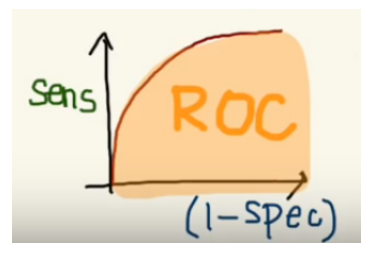
\includegraphics[width=0.8\linewidth]{roc6}
\end{center}

\tiny{(Ref: Let's learn about AUC ROC Curve! – GreyAtom)}
\end{column}

\end{columns}
\end{frame}




%%%%%%%%%%%%%%%%%%%%%%%%%%%%%%%%%%%%%%%%%%%%%%%%%%%%%%%%%%%%%%%%%%%%%%%%%
%\begin{frame}[fragile]\frametitle{``Default.csv'' Dataset}
%\begin{itemize}
%\item 10,000 observations
%
%\item 4 variables
%	\begin{itemize}
%	\item Default: ${Yes, No}$ - whether customer defaulted on their debt
%	\item Student: ${Yes, No}$ - whether customer is a student
%	\item Balance: average CC balance
%	\item Income: customer income
%	\end{itemize}
%
%\item Considering Balance as feature and Default as outcome, $\beta_1 = 0.0047$
%\end{itemize}
%%\begin{lstlisting}
%%reg = linear_model.LogisticRegression()
%%reg.fit(default['balance'].reshape(-1,1), default['default'])
%%Coefficients: [[ 0.00478248]]
%%Intercept: [-9.46506555] 
%%\end{lstlisting}
%A one-unit increase in balance is associated with an increase in the log odds of default by 0.0047 units.
%\end{frame}
%
%%%%%%%%%%%%%%%%%%%%%%%%%%%%%%%%%%%%%%%%%%%%%%%%%%%%%%%%%%%%%%%%%%%%%%%%%
%\begin{frame}[fragile]\frametitle{Making Predictions}
%For different Balance(s) what are the chances of Default?
%\begin{center}
%
\includegraphics[width=\linewidth]{predlog}
%\end{center}
%Find : Do students have a higher chance of default?
%\end{frame}

% %%%%%%%%%%%%%%%%%%%%%%%%%%%%%%%%%%%%%%%%%%%%%%%%%%%%%%%%%%%%%%%%%%%%%%%%%%%%%%%%%%
% \begin{frame}[fragile]\frametitle{}
% \begin{center}
% {\Large Evaluation Metrics: ROC AUC}
% \end{center}
% \end{frame}

%%%%%%%%%%%%%%%%%%%%%%%%%%%%%%%%%%%%%%%%%%%%%%%%%%%%%%%%%%%%%%%%%%%%%%%%
\begin{frame}[fragile]\frametitle{ROC AUC Intuition (More Details)}

\begin{columns}
\begin{column}[T]{0.5\linewidth}
\begin{itemize}
\item ROC : Receiver Operating Characteristics Curve
\item AUC: Area under curve
\item Often used to evaluate performance of a binary classifier
\item Two possible outcomes: Positive and Negative
\item This is histogram (continuous) where red pixels are positive (got admission to IIT!!) and blue pixels are negative (did not get admitted)
\item 250 students (pixels here, for example) got admitted and 250 did not get admitted.
\end{itemize}
\end{column}
\begin{column}[T]{0.5\linewidth}

\begin{center}
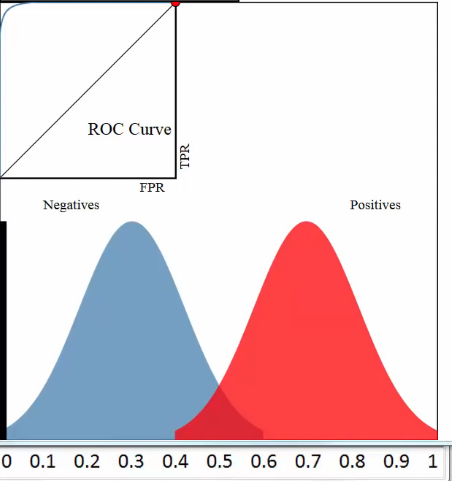
\includegraphics[width=0.9\linewidth]{binclass1}
\end{center}

\tiny{(Ref: ROC Curves and Area Under the Curve (AUC) Explained - Data School)}
\end{column}

\end{columns}
\end{frame}

%%%%%%%%%%%%%%%%%%%%%%%%%%%%%%%%%%%%%%%%%%%%%%%%%%%%%%%%%%%%%%%%%%%%%%%%
\begin{frame}[fragile]\frametitle{ROC AUC Intuition}

\begin{columns}
\begin{column}[T]{0.5\linewidth}
\begin{itemize}
\item This is result of predictions done on validation set. For which, you have actual values as well.
\item The classifier is like Logistic Regression where you get probabilities as well.
\item Predicted probabilities are seen on the x axis. Y axis is count of students with ACTUAL red(admitted) or blue (not admitted) values
\item E.g. there were 10 students for which you predicted admission probability of 0.1, they did not get admitted shown as negative (blue)
\end{itemize}
\end{column}
\begin{column}[T]{0.5\linewidth}

\begin{center}
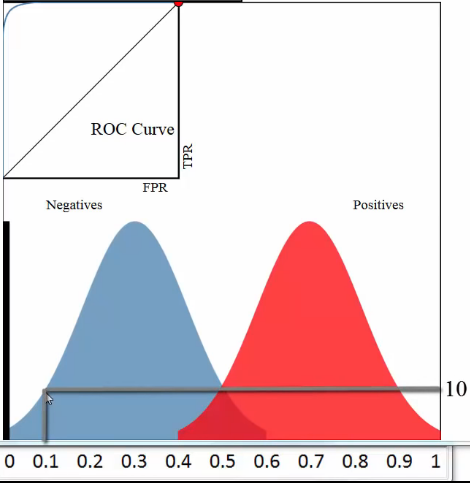
\includegraphics[width=0.9\linewidth]{binclass2}
\end{center}

\tiny{(Ref: ROC Curves and Area Under the Curve (AUC) Explained - Data School)}
\end{column}

\end{columns}
\end{frame}

%%%%%%%%%%%%%%%%%%%%%%%%%%%%%%%%%%%%%%%%%%%%%%%%%%%%%%%%%%%%%%%%%%%%%%%%
\begin{frame}[fragile]\frametitle{ROC AUC Intuition}

\begin{columns}
\begin{column}[T]{0.5\linewidth}
\begin{itemize}
\item E.g. there were 50 students for which you predicted admission probability of 0.3, they did not get admitted, ie negative (blue) (not shown here, but height of the bell curve is 50 )
\item For 20 students where you predicted 0.5 probability of admission, 10 did not get admitted (blue) but 10 got admitted (red)
\item You can say that the classifier is doing well as it is able to partition/separate two classes reasonably well (only small overlap or ambiguity in the middle)
\end{itemize}
\end{column}
\begin{column}[T]{0.5\linewidth}

\begin{center}
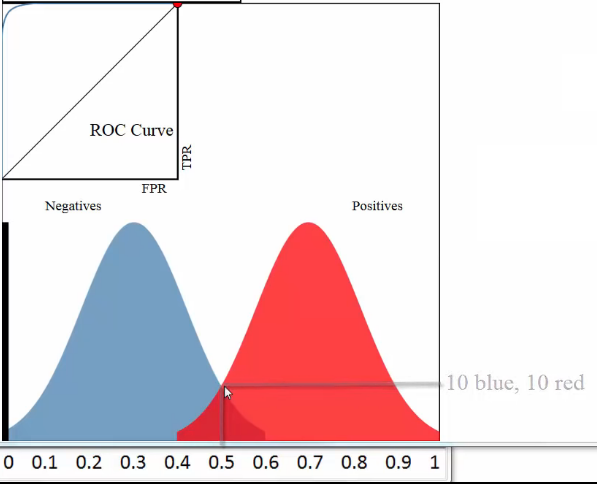
\includegraphics[width=0.9\linewidth]{binclass3}
\end{center}

\tiny{(Ref: ROC Curves and Area Under the Curve (AUC) Explained - Data School)}
\end{column}

\end{columns}
\end{frame}

%%%%%%%%%%%%%%%%%%%%%%%%%%%%%%%%%%%%%%%%%%%%%%%%%%%%%%%%%%%%%%%%%%%%%%%%
\begin{frame}[fragile]\frametitle{ROC AUC Intuition}

\begin{columns}
\begin{column}[T]{0.5\linewidth}
\begin{itemize}
\item So. we can put threshold (or the partition) at 0.5, anything about that is admitted, and below is not admitted.
\item With this threshold the accuracy looks to be in the range of 90\%.
\item Please not that the ROC curve in the top left is almost touching the left and top boundaries. Its bit away at the corner due to some errors in the middle region.
\end{itemize}
\end{column}
\begin{column}[T]{0.5\linewidth}

\begin{center}
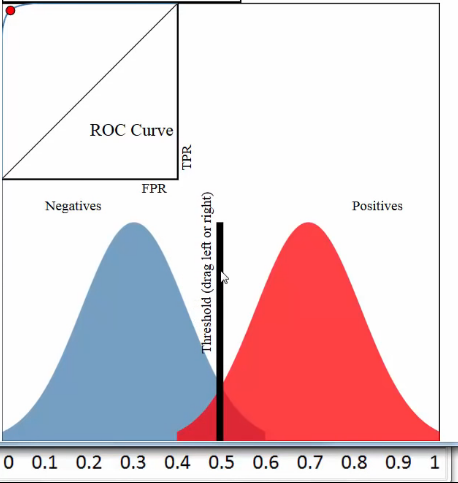
\includegraphics[width=0.9\linewidth]{binclass4}
\end{center}

\tiny{(Ref: ROC Curves and Area Under the Curve (AUC) Explained - Data School)}
\end{column}

\end{columns}
\end{frame}

%%%%%%%%%%%%%%%%%%%%%%%%%%%%%%%%%%%%%%%%%%%%%%%%%%%%%%%%%%%%%%%%%%%%%%%%
\begin{frame}[fragile]\frametitle{ROC AUC Intuition}

\begin{columns}
\begin{column}[T]{0.5\linewidth}
\begin{itemize}
\item If the classifier was not good, there would be far more overlap in the middle,ie many misclassifications.
\item Regardless of where you put threshold, your classification accuracy will be bad
\item Note that the ROC curve has shifted and too much gap way from the top left corner, so many errors.
\item ROC curve is a plot of True Positive Rate (TPR) on y axis and False Positive Rate (FPR) on x axis for every possible classification threshold (say, 0 to 1)
\end{itemize}
\end{column}
\begin{column}[T]{0.5\linewidth}

\begin{center}
\includegraphics[width=0.9\linewidth]{binclass5}
\end{center}

\tiny{(Ref: ROC Curves and Area Under the Curve (AUC) Explained - Data School)}
\end{column}

\end{columns}
\end{frame}

%%%%%%%%%%%%%%%%%%%%%%%%%%%%%%%%%%%%%%%%%%%%%%%%%%%%%%%%%%%%%%%%%%%%%%%%
\begin{frame}[fragile]\frametitle{ROC AUC Intuition}

\begin{columns}
\begin{column}[T]{0.5\linewidth}
\begin{itemize}
\item TPR : True Positives Predicted divided by All actual positives
\item FPR : False Positives Predicted divided by All actual negatives
\item Both range from 0 to 1.
\item For threshold 0.8, TPR is pixels on right (approx 50) divided by all reds (actual positives) ie 250, so $50/250 = 0.2$,
\item FPR is blue pixels on right of the line (0) divided by all blues ie 250, so $0/250 = 0$
\item Plot point at x = 0, and y = 0.2
\end{itemize}
\end{column}
\begin{column}[T]{0.5\linewidth}

\begin{center}
\includegraphics[width=0.9\linewidth]{binclass6}
\end{center}

\tiny{(Ref: ROC Curves and Area Under the Curve (AUC) Explained - Data School)}
\end{column}

\end{columns}
\end{frame}


%%%%%%%%%%%%%%%%%%%%%%%%%%%%%%%%%%%%%%%%%%%%%%%%%%%%%%%%%%%%%%%%%%%%%%%%
\begin{frame}[fragile]\frametitle{ROC AUC Intuition}

\begin{columns}
\begin{column}[T]{0.5\linewidth}
\begin{itemize}
\item For threshold 0.5, TPR is pixels on right (approx 230) divided by all reds (actual positives) ie 250, so $230/250 = 0.94$,
\item FPR is blue pixels on right of the line (125) divided by all blues ie 250, so $125/250 = 0.5$
\item Plot point at x = 0.5, and y = 0.94
\end{itemize}
\end{column}
\begin{column}[T]{0.5\linewidth}

\begin{center}
\includegraphics[width=0.9\linewidth]{binclass7}
\end{center}

\tiny{(Ref: ROC Curves and Area Under the Curve (AUC) Explained - Data School)}
\end{column}

\end{columns}
\end{frame}

%%%%%%%%%%%%%%%%%%%%%%%%%%%%%%%%%%%%%%%%%%%%%%%%%%%%%%%%%%%%%%%%%%%%%%%%
\begin{frame}[fragile]\frametitle{ROC AUC Intuition}

\begin{columns}
\begin{column}[T]{0.5\linewidth}
\begin{itemize}
\item Similarly plot for all possible thresholds. 
\item Thus ROC curve visualizes all possible thresholds.
\item It shows how the classifier is AWAY from the ideal, top left corner
\item The worst classier would be the diagonal straight line.  50\% line ie random chance.
\item So, to distinguish good classifier from a bad one, Area Under Curve is used.
\end{itemize}
\end{column}
\begin{column}[T]{0.5\linewidth}

\begin{center}
\includegraphics[width=0.9\linewidth]{binclass8}
\end{center}

\tiny{(Ref: ROC Curves and Area Under the Curve (AUC) Explained - Data School)}
\end{column}

\end{columns}
\end{frame}

%%%%%%%%%%%%%%%%%%%%%%%%%%%%%%%%%%%%%%%%%%%%%%%%%%%%%%%%%%%%%%%%%%%%%%%%
\begin{frame}[fragile]\frametitle{ROC AUC Intuition}

\begin{columns}
\begin{column}[T]{0.5\linewidth}
\begin{itemize}
\item AUC is Area under ROC curve divided by the whole square, say 0.8 for this example.
\item A poor classifier (diagonal line) will have area 0.5
\item Best classifier will be (corner legs) will have area 1.
\item Note that the Class labels are balanced in this example, ie number of students admitted and not admitted is roughly equal), so heights of the bell curves are same. That does not affect ROC AUC calculations though.
\item Choosing threshold is a business decision.
\end{itemize}
\end{column}
\begin{column}[T]{0.5\linewidth}

\begin{center}
\includegraphics[width=0.9\linewidth]{binclass9}
\end{center}

\tiny{(Ref: ROC Curves and Area Under the Curve (AUC) Explained - Data School)}
\end{column}

\end{columns}
\end{frame}


% %%%%%%%%%%%%%%%%%%%%%%%%%%%%%%%%%%%%%%%%%%%%%%%%%%%%%%%%%%%%%%%%%%%%%%%%
% \begin{frame}[fragile]\frametitle{ROC AUC Example}
% Lets look at one example:

% \begin{itemize}

% \item Form a table with y as actual values and $P_+$ predictions probabilities as given by logistic regression.
% \item So, for 1s we will get close to 1 probabilities and for 0s, close to 0.
% \item 3rd example shown is for error.
% \item Sort on Probabilities, like ranking or scoring.
% \end{itemize}

% \begin{center}
% \includegraphics[width=0.35\linewidth]{cf1}
% \end{center}
% \end{frame}

% %%%%%%%%%%%%%%%%%%%%%%%%%%%%%%%%%%%%%%%%%%%%%%%%%%%%%%%%%%%%%%%%%%%%%%%%
% \begin{frame}[fragile]\frametitle{ROC AUC Example}

% \begin{itemize}
% \item Decide a threshold and partition the sorted column 
% \item New column for Predictions where value above partition are 1s and below, 0s.
% \item Decide following terms:
% \begin{itemize}
% \item True Positive Rate (TPR or Recall) $\frac{TP}{TP+FN}$ (shown magenta)
% \item False Positive Rate (FPR) $\frac{FP}{FP+TN}$ (shown red)
% \end{itemize}
% \end{itemize}

% \begin{center}
% \includegraphics[width=0.8\linewidth]{cf2}
% \end{center}
% \end{frame}

% %%%%%%%%%%%%%%%%%%%%%%%%%%%%%%%%%%%%%%%%%%%%%%%%%%%%%%%%%%%%%%%%%%%%%%%%
% \begin{frame}[fragile]\frametitle{ROC AUC Example}

% \begin{itemize}
% \item Vary threshold to get different TPR and FPR
% \item Plot the points with FPR on x and TPR on y, for different thresholds.
% \item Ideal would be with TPR = 1 and FPR = 0. The y axis point. So the whole rectangle is the full area.
% \item Practical is of course less than ideal, as seen. $\frac{8}{9}$
% \item AUC as 0.5 is like random classification. The baseline where TPR and FPR are equal.
% \end{itemize}

% \begin{center}
% \includegraphics[width=0.65\linewidth]{cf3}
% \end{center}
% \end{frame}

% %%%%%%%%%%%%%%%%%%%%%%%%%%%%%%%%%%%%%%%%%%%%%%%%%%%%%%%%%%%%%%%%%%%%%%%%
% \begin{frame}[fragile]\frametitle{ROC AUC Example}

% % \begin{center}
% % \includegraphics[width=0.3\linewidth]{logistic4}
% % \end{center}

% \begin{itemize}
% \item AUC interpretation: If you pick random positive example and a negative one, whats the probability that my model will give higher score to positive (meaning correct class identification) than to the negative.
% \item That value is the area under curve. If its 0.9, thats the probability of getting correct class identification.
% \item Intuition: gives an aggregate measure of performance aggregated across all possible classification thresholds.
% % \item Not IDEAL measure. If errors are more, it calculates misclassification as ROC AUC and thats wrong. (??)
% \end{itemize}
% \end{frame}


% %%%%%%%%%%%%%%%%%%%%%%%%%%%%%%%%%%%%%%%%%%%%%%%%%%%%%%%%%%
% \begin{frame}[fragile]\frametitle{ROC AUC (Recap)}
% \begin{center}
% \includegraphics[width=0.9\linewidth,keepaspectratio]{confmat12}
% \end{center}
% \tiny{(Reference: Introduction to Machine Learning - Andrew Ng)}
% \end{frame}


%%%%%%%%%%%%%%%%%%%%%%%%%%%%%%%%%%%%%%%%%%%%%%%%%%%%%%%%%%%%%%%%%%%%%%%%%%%%%%%%%%
\begin{frame}[fragile]\frametitle{}
\begin{center}
{\Large Complex Variations}
\end{center}
\end{frame}



%%%%%%%%%%%%%%%%%%%%%%%%%%%%%%%%%%%%%%%%%%%%%%%%%%%%%%%%%%%%%%%%%%%%%%%%
\begin{frame}[fragile]\frametitle{Multiple Xs Logistic Regression}
\begin{itemize}
\item How to prediction a binary response using multiple predictors?
\item Can generalize the logistic function to p predictors
\end{itemize}
\begin{center}
\includegraphics[width=\linewidth]{multilog}
\end{center}
%Can use maximum likelihood to estimate the $p+1$ coefficients?
\end{frame}

%%%%%%%%%%%%%%%%%%%%%%%%%%%%%%%%%%%%%%%%%%%%%%%%%%%%%%%%%%%%%%%%%%%%%%%%%
% \begin{frame}[fragile]\frametitle{Multiple Xs Logistic Regression}
% \begin{itemize}
%\item It predicts the probability, its output values lies between 0 and 1 (as expected).
%$logit(p) = \log(p/(1-p)) = b_0 + b_1 x_1 +  \ldots + b_k x_k$
%\item Above, p is the probability of presence of the characteristic of interest. It chooses parameters that maximize  the  likelihood  of  observing  the  sample  values  rather  than  that  minimize  the  sum  of squared errors (like in ordinary regression).
%\end{itemize}
%\end{frame}

%%%%%%%%%%%%%%%%%%%%%%%%%%%%%%%%%%%%%%%%%%%%%%%%%%%%%%%%%%%%%%%%%%%%%%%%
\begin{frame}[fragile]\frametitle{Multi Class Classification}
\begin{itemize}
\item Example: Email tagging: Work, Friends, Family, Hobby.
\item 4 class problem: y = 1 or 2 or 3 or 4
\item Other Example: Weather: Sunny, Cloudy, Rainy, Snow
\item Target has discrete values (int)
\end{itemize}
\end{frame}

%%%%%%%%%%%%%%%%%%%%%%%%%%%%%%%%%%%%%%%%%%%%%%%%%%%%%%%%%%%%%%%%%%%%%%%%
\begin{frame}[fragile]\frametitle{Multi Class Logistic Regression}
\begin{itemize}
\item How to prediction a multi-class response?
\item Can generalize the logistic function to n targets?
\item One vs All
\end{itemize}
\end{frame}

%%%%%%%%%%%%%%%%%%%%%%%%%%%%%%%%%%%%%%%%%%%%%%%%%%%%%%%%%%%%%%%%%%%%%%%%
\begin{frame}[fragile]\frametitle{One Vs All (or Rest)}
\begin{itemize}
\item Separate classification problems
\item One class variable vs Not-that-Class
\item Do this for all target variables
\end{itemize}
\begin{center}
\includegraphics[width=0.8\linewidth]{logregf3}
\end{center}
\tiny{(Reference: Simple Linear Regression: Step-By-Step - Dan Wellisch)}
\end{frame}

%%%%%%%%%%%%%%%%%%%%%%%%%%%%%%%%%%%%%%%%%%%%%%%%%%%%%%%%%%%%%%%%%%%%%%%%
\begin{frame}[fragile]\frametitle{One Vs All (or Rest)}
\begin{itemize}
\item Each classifier gives its probability of its target class
\item We take MAX among them
\end{itemize}
\begin{center}
\includegraphics[width=0.8\linewidth]{logregf4}
\end{center}
\end{frame}


%%%%%%%%%%%%%%%%%%%%%%%%%%%%%%%%%%%%%%%%%%%%%%%%%%%%%%%%%%%%%%%%%%%%%%%%%
%\begin{frame}[fragile]\frametitle{Full Model}
%\begin{itemize}
%\item RESPONSE/OUTCOME: Default: {Yes, No} - whether customer defaulted on their debt
%\item PREDICTORS/FEATURES:
%	\begin{itemize}
%	\item (DUMMY VARIABLE USED) Student: {Yes, No} - whether customer is a student
%	\item Balance: average CC balance
%	\item Income: customer income
%	\end{itemize}
%\end{itemize}
%\begin{lstlisting}
%Predictor Names: Index(['balance', 'income', 'student_Yes'], dtype='object') 
%Coefficients: [[ 4.07585063e-04 -1.25881574e-04 -2.51032533e-06]] 
%Intercept: [ -1.94180590e-06] 
%\end{lstlisting}
%Coefficient for the dummy variable student is negative, indicating that students are less likely to default than nonstudents.
%\end{frame}
%
%%%%%%%%%%%%%%%%%%%%%%%%%%%%%%%%%%%%%%%%%%%%%%%%%%%%%%%%%%%%%%%%%%%%%%%%%
%\begin{frame}[fragile]\frametitle{Interpretation is Key}
%\begin{itemize}
%\item In linear regression, results obtained using one predictor may be vastly different compared to when multiple predictors are used
%Especially when there is correlation among the predictors
%\item Default rate of students/non-students, as a function of balance value
%\item A student is less likely to default than a non-student, for a fixed value of balance.
%\end{itemize}
%\begin{center}
%\includegraphics[width=0.5\linewidth]{intlog}
%\end{center}
%\end{frame}
%
%
%%%%%%%%%%%%%%%%%%%%%%%%%%%%%%%%%%%%%%%%%%%%%%%%%%%%%%%%%%%%%%%%%%%%%%%%%
%\begin{frame}[fragile]\frametitle{Encoding}
%\begin{itemize}
%\item Iris dataset: outcome variable is flower type : {Setosa, Virginica, Versicolor}
%\item For training if we encode as {1,2,3} respectively, fit linear regression, is it correct?
%\item Encoding implies an ordering of the Iris classes
%\item Difference between Setosa and Virginica is same as difference between Viginica and Versicolor
%\item Difference between Setosa and Versicolor is greatest
%\item If order is changed, model changes, prediction changes for same test instance.
%\item In general, no natural way to convert a qualitative response with more than two levels into a quantitative response
%\item But for binary response? 0 for fail, 1 for success?
%\end{itemize}
%\end{frame}
%
%%%%%%%%%%%%%%%%%%%%%%%%%%%%%%%%%%%%%%%%%%%%%%%%%%%%%%%%%%%%%%%%%%%%%%%%%
%\begin{frame}[fragile]\frametitle{Binrary Outocme}
%\begin{itemize}
%\item Predict Failed if $y < 0.5$, Else predict Success.
%\item Predicted values may lie outside range of [0,1]
%\item Predicted values are not probabilities
%\item Logistic Regression models the probability that Y belongs to a particular category. 
%\item {\bf IT DOES NOT MODEL THE ACTUAL OUTCOME VALUE}
%\item Probability of Default given Balance: $p(Default = Yes | Balance)$
%\item If $p(default |balance) > 0.5$ then Predict Default=Yes
%\item For a conservative company threshold can be 0.1 instead of 0.5
%\end{itemize}
%\end{frame}
%
%%%%%%%%%%%%%%%%%%%%%%%%%%%%%%%%%%%%%%%%%%%%%%%%%%%%%%%%%%%%%%%%%%%%%%%%%%%%%%%%%%
\begin{frame}[fragile]\frametitle{}
\begin{center}
{\Large Summary}
\end{center}
\end{frame}

%%%%%%%%%%%%%%%%%%%%%%%%%%%%%%%%%%%%%%%%%%%%%%%%%%%%%%%%%%%%%%%%%%%%%%%%
\begin{frame}[fragile]\frametitle{Regression vs. Classification}
\begin{itemize}
\item In standard linear regression, the response is a continuous variable (float). It can take any value, large/small, positive/negative, integer/float, etc.
\item In logistic regression, the response is qualitative/discrete (int, enum)
\item Binary responses: Success or failure, Spam or Ham (Not Spam), etc They are bound to only categorical values such as 0,1.
\item Its like converting analog signal (values, any float number) to digital signal (0 and 1s only)
%\item How do we do that?
\item Note: Independent variables (Xs) can be of any type ie continuous or discrete, for both, Regression and Classification problems. They are differentiated based on the type of the target (y) only. If target is continuous then its a Regression problem and if the target is discrete then its a Classification problem.
\end{itemize}

\end{frame}


%%%%%%%%%%%%%%%%%%%%%%%%%%%%%%%%%%%%%%%%%%%%%%%%%%%%%%%%%%%%%%%%%%%%%%%%
\begin{frame}[fragile]\frametitle{Linear Model vs. Logistic Model}
\begin{center}
\includegraphics[width=\linewidth]{loglin}
\end{center}
Logistic Function: outputs between 0 and 1 for all values of X

\end{frame}
